\documentclass[pdf]{beamer}

\usepackage{amsmath}
\usepackage{amsfonts}
\usepackage{amssymb}
\usepackage{amsthm}
\usepackage[english]{babel}
\usepackage{mathtools}
\usepackage{verbatim}
\usepackage{tikz}
\usepackage[ruled,vlined]{algorithm2e}
\usepackage[parfill]{parskip}

\mode<presentation>{}

%\usecolortheme{orchid}

\title{Implementing algorithms for path 3-coloring and path 3-list-coloring
	plane graphs}
\subtitle{Final Talk}
\author{Aven Bross}
\date{February 28, 2017}

\theoremstyle{definition}
\newtheorem{thm}{Theorem}

\theoremstyle{definition}
\newtheorem{pf}{Proof}

\theoremstyle{definition}
\newtheorem{dfn}{Definition}

\theoremstyle{definition}
\newtheorem{prb}{Problem}

\theoremstyle{definition}
\newtheorem{sol}{Solution}

\theoremstyle{definition}
\newtheorem{imp}{Implementation}

\theoremstyle{definition}
\newtheorem{rmk}{Note}

\theoremstyle{definition}
\newtheorem{exm}{Example}

\theoremstyle{definition}
\newtheorem{ida}{Idea}

\theoremstyle{definition}
\newtheorem{alg}{Algorithm}

\theoremstyle{definition}
\newtheorem{stp}{Step}

\theoremstyle{definition}
\newtheorem{cse}{Case}

\tikzset{
    every node/.style={circle, fill, draw, minimum size=1mm, scale=.8,
    	font=\LARGE}
}

\tikzset{
    every edge/.append style={line width=1.5pt}
}

\tikzset{
	every loop/.style={min distance=3cm,in=-15,out=45,looseness=15}
}

\pgfdeclarelayer{background}
\pgfsetlayers{background,main}

\AtBeginSection[]
{
	\begin{frame}{Overview}
	\tableofcontents[currentsection]
	\end{frame}
}

\begin{document}

%% title frame
\begin{frame}
\titlepage
\end{frame}

\begin{frame}{Committee}
\begin{itemize}
	\item Dr. Chappell (Chair)
	\item Dr. Lawlor
	\item Dr. Hartman
\end{itemize}
\end{frame}

\begin{frame}{Project goal}
Produce a nice, documented implementation of two previously unimplemented
algorithms for coloring planar graphs.
\end{frame}

\section{Plane graphs}

\begin{frame}{Graphs}
A \textbf{graph} consists of:
\begin{enumerate}
	\item a set of objects called \textbf{vertices};
\end{enumerate}
\hfill\\
\hfill\\

\begin{center}
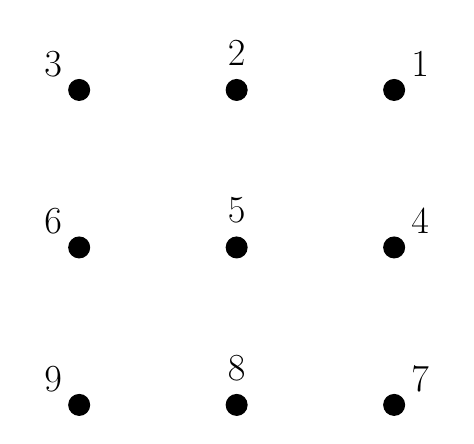
\begin{tikzpicture}
	\node (1) [label=above right:{1}] at ( 2.0cm,  2.0cm) {};
	\node (2) [label=above:{2}] at ( 0.0cm,  2.0cm) {};
	\node (3) [label=above left:{3}] at (-2.0cm,  2.0cm) {};
	\node (4) [label=above right:{4}] at ( 2.0cm,  0.0cm) {};
	\node (5) [label=above:{5}] at ( 0.0cm,  0.0cm) {};
	\node (6) [label=above left:{6}] at (-2.0cm,  0.0cm) {};
	\node (7) [label=above right:{7}] at ( 2.0cm, -2.0cm) {};
	\node (8) [label=above:{8}] at ( 0.0cm, -2.0cm) {};
	\node (9) [label=above left:{9}] at (-2.0cm, -2.0cm) {};
\end{tikzpicture}
\end{center}
\end{frame}

\begin{frame}{Graphs}
A \textbf{graph} consists of:
\begin{enumerate}
	\item a set of objects called \textbf{vertices};
	\item a set of \textbf{edges} between pairs of vertices.
\end{enumerate}
\hfill\\

\begin{center}
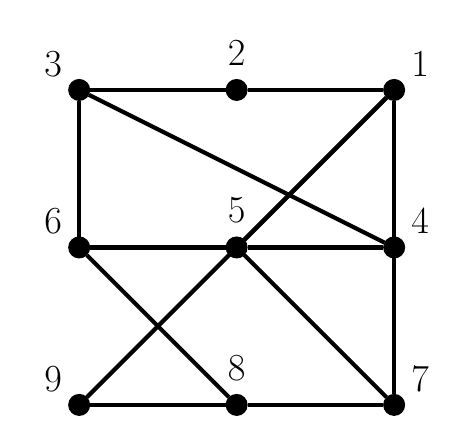
\begin{tikzpicture}
	\node (1) [label=above right:{1}] at ( 2.0cm,  2.0cm) {};
	\node (2) [label=above:{2}] at ( 0.0cm,  2.0cm) {};
	\node (3) [label=above left:{3}] at (-2.0cm,  2.0cm) {};
	\node (4) [label=above right:{4}] at ( 2.0cm,  0.0cm) {};
	\node (5) [label=above:{5}] at ( 0.0cm,  0.0cm) {};
	\node (6) [label=above left:{6}] at (-2.0cm,  0.0cm) {};
	\node (7) [label=above right:{7}] at ( 2.0cm, -2.0cm) {};
	\node (8) [label=above:{8}] at ( 0.0cm, -2.0cm) {};
	\node (9) [label=above left:{9}] at (-2.0cm, -2.0cm) {};
	
	\draw (2) edge (1); \draw (3) edge (6);
	\draw (6) edge (8); \draw (2) edge (3);
	\draw (8) edge (9); \draw (9) edge (1);
	\draw (7) edge (5); \draw (1) edge (5);
	\draw (8) edge (7); \draw (4) edge (7);
	\draw (1) edge (4); \draw (3) edge (4);
	\draw (4) edge (5); \draw (5) edge (6);
\end{tikzpicture}
\end{center}
\end{frame}

\begin{frame}{Simple graphs}
All graphs in this talk will be \textbf{simple} graphs which have no
\textbf{loops} or \textbf{parallel edges}.\\

\begin{center}
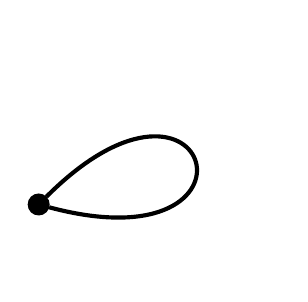
\begin{tikzpicture}
  \node (a) at (0cm,-0.25cm) {};
  \node [fill=none,draw=none] at (0cm, -1cm) {};
  
  \draw (a) edge [loop above] (a);
\end{tikzpicture}
$\qquad$
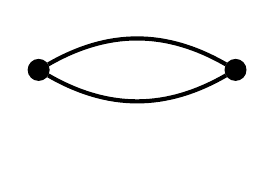
\begin{tikzpicture}
  \node (a) at (0cm,0cm) {};
  \node (b) at (2.5cm,0cm) {};
  \node [fill=none,draw=none] at (0cm, -1cm) {};
  
  \draw (a) edge [bend right] (b);
  \draw (a) edge [bend left] (b);
\end{tikzpicture}\\
\hfill\\
\footnotesize{A loop (left) and two parallel edges (right).}
\end{center}
\end{frame}

\begin{frame}{Plane graphs}
We are interested in \textbf{planar graphs} which are graphs that may be drawn
in the plane without crossing edges. A planar graph along with a particular
drawing is called a \textbf{plane graph}.\\
\hfill\\

\begin{center}
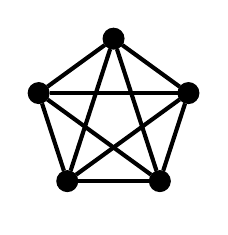
\begin{tikzpicture}
	\node (a) at (90:1cm) {};
	\node (b) at (162:1cm) {};
	\node (c) at (234:1cm) {};
	\node (d) at (306:1cm) {};
	\node (e) at (18:1cm) {};
	\node [draw=none, fill=none] (1) at (0cm,-1cm) {};
	\node [draw=none, fill=none] (2) at (0cm,1cm) {};
	\draw (a) edge (b); \draw (a) edge (c); \draw (a) edge (d); \draw (a) edge (e);
	\draw (b) edge (c); \draw (b) edge (d); \draw (b) edge (e); \draw (c) edge (d);
	\draw (c) edge (e); \draw (d) edge (e);
\end{tikzpicture}
$\qquad$
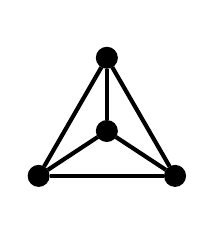
\begin{tikzpicture}
	\node (a) at (0cm,0.75cm) {};
	\node (b) at (0.866cm,-0.75cm) {};
	\node (c) at (-0.866cm,-0.75cm) {};
	\node (d) at (0cm, -0.18cm) {};
	\node [draw=none, fill=none] (1) at (0cm,-1cm) {};
	\node [draw=none, fill=none] (2) at (0cm,1cm) {};
	\draw (a) edge (b); \draw (b) edge (c); \draw (c) edge (d);
	\draw (d) edge (a); \draw (a) edge (c); \draw (b) edge (d);
\end{tikzpicture}\\
\hfill\\
\footnotesize{The nonplanar graph $K_5$, and the planar graph $K_4$.}
\end{center}
\end{frame}

\begin{frame}{Faces}
A \textbf{face} of a plane graph is a maximal region of the plane not containing
any edges or vertices.\\
\hfill\\

\begin{center}
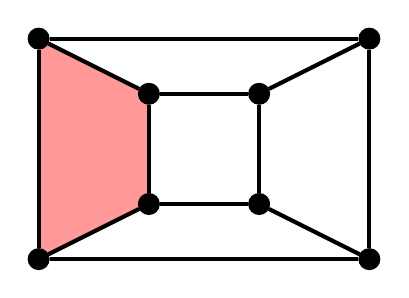
\begin{tikzpicture}[scale=0.7]
	\node (1) at (-3cm,2cm) {};
	\node (2) at (3cm,2cm) {};
	\node (3) at (3cm,-2cm) {};
	\node (4) at (-3cm,-2cm) {};
	\node (5) at (-1cm,1cm) {};
	\node (6) at (1cm,1cm) {};
	\node (7) at (1cm,-1cm) {};
	\node (8) at (-1cm,-1cm) {};
	
	\begin{pgfonlayer}{background}
		\fill[red!40] (-3cm,2cm) -- (-1cm, 1cm) -- (-1cm, -1cm)
			-- (-3cm,-2cm) -- cycle;
	\end{pgfonlayer}
	
	\draw (1) edge (2); \draw (2) edge (3); \draw (3) edge (4);
	\draw (4) edge (1);
	\draw (5) edge (6); \draw (6) edge (7); \draw (7) edge (8);
	\draw (8) edge (5);
	\draw (1) edge (5); \draw (2) edge (6); \draw (3) edge (7);
	\draw (4) edge (8);
\end{tikzpicture}
\end{center}
\end{frame}

\begin{frame}{Faces}
We will refer to a face by the subgraph of vertices and edges lying on its
border.\\
\hfill\\

\begin{center}
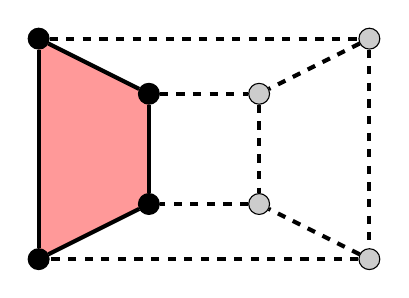
\begin{tikzpicture}[scale=0.7]
	\node (1) at (-3cm,2cm) {};
	\node (2) [fill opacity=0.2] at (3cm,2cm) {};
	\node (3) [fill opacity=0.2] at (3cm,-2cm) {};
	\node (4) at (-3cm,-2cm) {};
	\node (5) at (-1cm,1cm) {};
	\node (6) [fill opacity=0.2] at (1cm,1cm) {};
	\node (7) [fill opacity=0.2] at (1cm,-1cm) {};
	\node (8) at (-1cm,-1cm) {};
	
	\begin{pgfonlayer}{background}
		\fill[red!40] (-3cm,2cm) -- (-1cm, 1cm) -- (-1cm, -1cm)
			-- (-3cm,-2cm) -- cycle;
	\end{pgfonlayer}
	
	\draw (1) edge [dashed] (2); \draw (2) edge [dashed] (3); \draw (3) edge [dashed] (4);
	\draw (4) edge (1);
	\draw (5) edge [dashed] (6); \draw (6) edge [dashed] (7); \draw (7) edge [dashed] (8);
	\draw (8) edge (5);
	\draw (1) edge (5); \draw (2) edge [dashed] (6); \draw (3) edge [dashed] (7);
	\draw (4) edge (8);
\end{tikzpicture}
\end{center}
\end{frame}

\begin{frame}{Faces}
The unbounded region is also a face, known as the \textbf{outer face}.\\
\hfill\\

\begin{center}
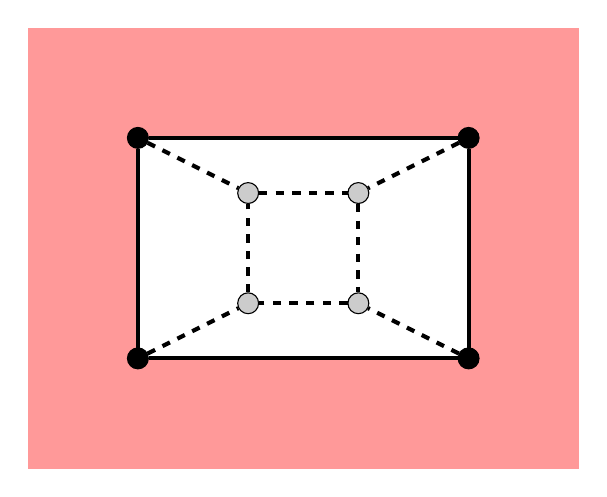
\begin{tikzpicture}[scale=0.7]
	\node (1) at (-3cm,2cm) {};
	\node (2) at (3cm,2cm) {};
	\node (3) at (3cm,-2cm) {};
	\node (4) at (-3cm,-2cm) {};
	\node (5) [fill opacity=0.2] at (-1cm,1cm) {};
	\node (6) [fill opacity=0.2] at (1cm,1cm) {};
	\node (7) [fill opacity=0.2] at (1cm,-1cm) {};
	\node (8) [fill opacity=0.2] at (-1cm,-1cm) {};
	
	\begin{pgfonlayer}{background}
		\fill[red!40] (-5cm,4cm) -- (5cm, 4cm) -- (5cm,2cm) -- (-5cm, 2cm)
			-- cycle;
		\fill[red!40] (-5cm,-4cm) -- (5cm, -4cm) -- (5cm,-2cm) -- (-5cm,-2cm)
			-- cycle;
		\fill[red!40] (-5cm,-3cm) -- (-5cm, 3cm) -- (-3cm,3cm) -- (-3cm,-3cm)
			-- cycle;
		\fill[red!40] (5cm,-3cm) -- (5cm, 3cm) -- (3cm,3cm) -- (3cm,-3cm)
			-- cycle;
	\end{pgfonlayer}
	
	\draw (1) edge (2); \draw (2) edge (3); \draw (3) edge (4);
	\draw (4) edge (1);
	\draw (5) edge [dashed] (6); \draw (6) edge [dashed] (7); \draw (7) edge [dashed] (8);
	\draw (8) edge [dashed] (5);
	\draw (1) edge [dashed] (5); \draw (2) edge [dashed] (6); \draw (3) edge [dashed] (7);
	\draw (4) edge [dashed] (8);
\end{tikzpicture}
\end{center}
\end{frame}

\begin{frame}{Triangulation}
A graph is \textbf{triangulated} if all of its faces are triangles. If a graph
has a single nontriangle face we say it is \textbf{weakly triangulated}.\\
\hfill\\

\begin{center}
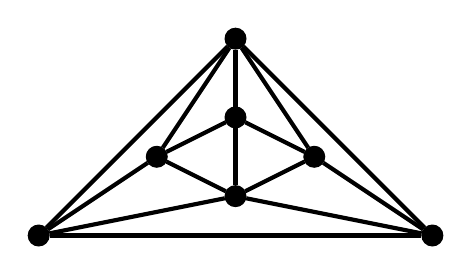
\begin{tikzpicture}[scale=.5]
  \node (0) at (0cm, 0cm) {};
  \node (1) at (7cm, 2cm) {};
  \node (2) at (10cm, 0cm) {};
  \node (3) at (3cm, 2cm) {};
  \node (4) at (5cm, 5cm) {};
  \node (5) at (5cm, 1cm) {};
  \node (6) at (5cm, 3cm) {};
  
  \draw (0) edge (2); \draw (2) edge (5); \draw (0) edge (5);
  \draw (3) edge (0); \draw (4) edge (6); \draw (5) edge (1);
  \draw (3) edge (6); \draw (2) edge (4); \draw (6) edge (1);
  \draw (4) edge (3); \draw (4) edge (0); \draw (1) edge (4);
  \draw (1) edge (2); \draw (5) edge (3); \draw (5) edge (6);
\end{tikzpicture}
$ \ $
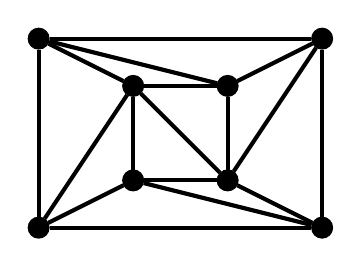
\begin{tikzpicture}[scale=0.6]
	\node (1) at (-3cm,2cm) {};
	\node (2) at (3cm,2cm) {};
	\node (3) at (3cm,-2cm) {};
	\node (4) at (-3cm,-2cm) {};
	\node (5) at (-1cm,1cm) {};
	\node (6) at (1cm,1cm) {};
	\node (7) at (1cm,-1cm) {};
	\node (8) at (-1cm,-1cm) {};
	
	\draw (1) edge (2); \draw (2) edge (3); \draw (3) edge (4);
	\draw (4) edge (1);
	\draw (5) edge (6); \draw (6) edge (7); \draw (7) edge (8);
	\draw (8) edge (5);
	\draw (1) edge (5); \draw (2) edge (6); \draw (3) edge (7);
	\draw (4) edge (8);
	\draw (4) edge (5); \draw (1) edge (6); \draw (2) edge (7);
	\draw (3) edge (8); \draw (5) edge (7);
\end{tikzpicture}\\
\hfill\\
\footnotesize{A triangulated graph and a weakly triangulated graph.}
\end{center}
\end{frame}

\begin{frame}{Rotation schemes}
A plane graph naturally provides a cyclic ordering of the edges around each
vertex, called a \textbf{rotation scheme}. In fact, the rotation scheme tells us
everything we need to know about the plane graph.\\
\hfill\\

\begin{center}
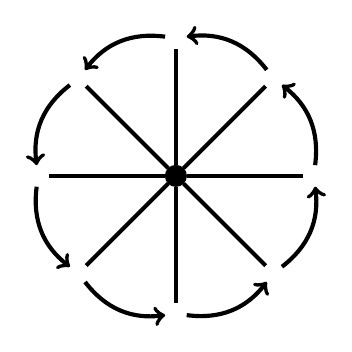
\begin{tikzpicture}
	\node (1) at (0:0cm) {};
	\node (2) [draw=none,fill=none] at (0:1.75cm) {};
	\node (3) [draw=none,fill=none] at (45:1.75cm) {};
	\node (4) [draw=none,fill=none] at (90:1.75cm) {};
	\node (5) [draw=none,fill=none] at (135:1.75cm) {};
	\node (6) [draw=none,fill=none] at (180:1.75cm) {};
	\node (7) [draw=none,fill=none] at (225:1.75cm) {};
	\node (8) [draw=none,fill=none] at (270:1.75cm) {};
	\node (9) [draw=none,fill=none] at (315:1.75cm) {};
	
	\draw (1) edge (2); \draw (1) edge (3); \draw (1) edge (4); \draw (1) edge (5);
	\draw (1) edge (6); \draw (1) edge (7); \draw (1) edge (8); \draw (1) edge (9);
	\draw (2) edge [->, bend right] (3); \draw (3) edge [->, bend right] (4);
	\draw (4) edge [->, bend right] (5); \draw (5) edge [->, bend right] (6);
	\draw (6) edge [->, bend right] (7); \draw (7) edge [->, bend right] (8);
	\draw (8) edge [->, bend right] (9); \draw (9) edge [->, bend right] (2);
\end{tikzpicture}
\end{center}
\end{frame}

\begin{frame}{Induced subgraphs}
Given a subset $S$ of vertices of a graph $G$, the \textbf{induced subgraph} of
$S$ consists of all edges in $G$ between vertices in $S$.\\
\hfill\\

\begin{center}
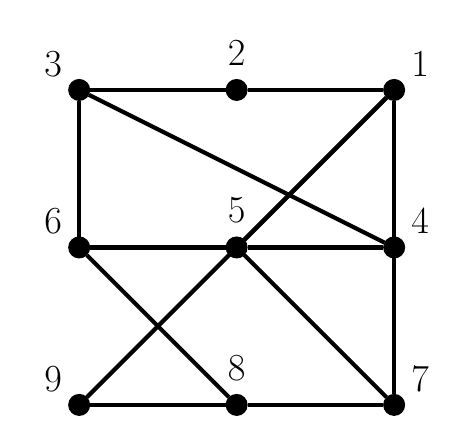
\begin{tikzpicture}
	\node (1) [label=above right:{1}] at ( 2.0cm,  2.0cm) {};
	\node (2) [label=above:{2}] at ( 0.0cm,  2.0cm) {};
	\node (3) [label=above left:{3}] at (-2.0cm,  2.0cm) {};
	\node (4) [label=above right:{4}] at ( 2.0cm,  0.0cm) {};
	\node (5) [label=above:{5}] at ( 0.0cm,  0.0cm) {};
	\node (6) [label=above left:{6}] at (-2.0cm,  0.0cm) {};
	\node (7) [label=above right:{7}] at ( 2.0cm, -2.0cm) {};
	\node (8) [label=above:{8}] at ( 0.0cm, -2.0cm) {};
	\node (9) [label=above left:{9}] at (-2.0cm, -2.0cm) {};
	
	\draw (2) edge (1); \draw (3) edge (6);
	\draw (6) edge (8); \draw (2) edge (3);
	\draw (8) edge (9); \draw (9) edge (1);
	\draw (7) edge (5); \draw (1) edge (5);
	\draw (8) edge (7); \draw (4) edge (7);
	\draw (1) edge (4); \draw (3) edge (4);
	\draw (4) edge (5); \draw (5) edge (6);
\end{tikzpicture}
\end{center}
\end{frame}

\begin{frame}{Induced subgraphs}
Given a subset $S$ of vertices of a graph $G$, the \textbf{induced subgraph} of
$S$ consists of all edges in $G$ between vertices in $S$.\\
\hfill\\
\begin{center}
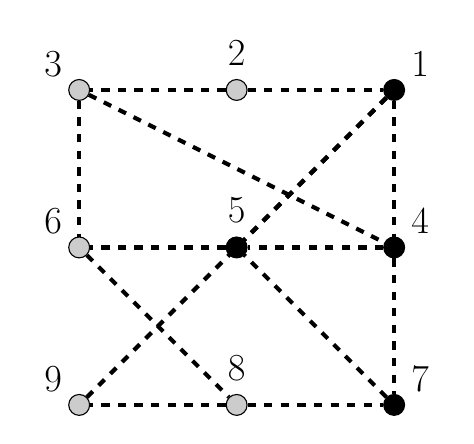
\begin{tikzpicture}
	\node (1) [label=above right:{1}] at ( 2.0cm,  2.0cm) {};
	\node (2) [label=above:{2}, fill opacity=0.2] at ( 0.0cm,  2.0cm) {};
	\node (3) [label=above left:{3}, fill opacity=0.2] at (-2.0cm,  2.0cm) {};
	\node (4) [label=above right:{4}] at ( 2.0cm,  0.0cm) {};
	\node (5) [label=above:{5}] at ( 0.0cm,  0.0cm) {};
	\node (6) [label=above left:{6}, fill opacity=0.2] at (-2.0cm,  0.0cm) {};
	\node (7) [label=above right:{7}] at ( 2.0cm, -2.0cm) {};
	\node (8) [label=above:{8}, fill opacity=0.2] at ( 0.0cm, -2.0cm) {};
	\node (9) [label=above left:{9}, fill opacity=0.2] at (-2.0cm, -2.0cm) {};
	
	\draw (2) edge (1) [dashed]; \draw (3) edge (6) [dashed];
	\draw (6) edge (8) [dashed]; \draw (2) edge (3) [dashed];
	\draw (8) edge (9) [dashed]; \draw (9) edge (1) [dashed];
	\draw (7) edge (5) [dashed]; \draw (1) edge (5) [dashed];
	\draw (8) edge (7) [dashed]; \draw (4) edge (7) [dashed];
	\draw (1) edge (4) [dashed]; \draw (3) edge (4) [dashed];
	\draw (4) edge (5) [dashed]; \draw (5) edge (6) [dashed];
\end{tikzpicture}
\end{center}
\end{frame}

\begin{frame}{Induced subgraphs}
Given a subset $S$ of vertices of a graph $G$, the \textbf{induced subgraph} of
$S$ consists of all edges in $G$ between vertices in $S$.\\
\hfill\\

\begin{center}
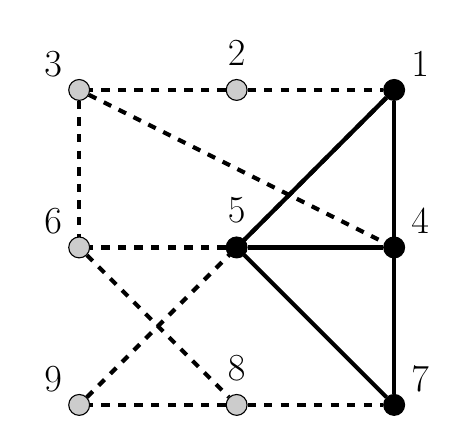
\begin{tikzpicture}
	\node (1) [label=above right:{1}] at ( 2.0cm,  2.0cm) {};
	\node (2) [label=above:{2}, fill opacity=0.2] at ( 0.0cm,  2.0cm) {};
	\node (3) [label=above left:{3}, fill opacity=0.2] at (-2.0cm,  2.0cm) {};
	\node (4) [label=above right:{4}] at ( 2.0cm,  0.0cm) {};
	\node (5) [label=above:{5}] at ( 0.0cm,  0.0cm) {};
	\node (6) [label=above left:{6}, fill opacity=0.2] at (-2.0cm,  0.0cm) {};
	\node (7) [label=above right:{7}] at ( 2.0cm, -2.0cm) {};
	\node (8) [label=above:{8}, fill opacity=0.2] at ( 0.0cm, -2.0cm) {};
	\node (9) [label=above left:{9}, fill opacity=0.2] at (-2.0cm, -2.0cm) {};
	
	\draw (2) edge (1) [dashed]; \draw (3) edge (6) [dashed];
	\draw (6) edge (8) [dashed]; \draw (2) edge (3) [dashed];
	\draw (8) edge (9) [dashed]; \draw (9) edge (1) [dashed];
	\draw (7)edge (5); \draw (1) edge (5);
	\draw (8) edge (7) [dashed];
	\draw (1) edge (4); \draw (3) edge (4) [dashed];
	\draw (4) edge (5); \draw (4) edge (7); \draw (5) edge (6) [dashed];
\end{tikzpicture}
\end{center}
\end{frame}

\begin{frame}{Paths}
A \textbf{path} is a sequence of distinct vertices with edges between consecutive
vertices.

A \textbf{cycle} consists of a path and an edge between the first and last
vertex.\\
\hfill\\

\begin{center}
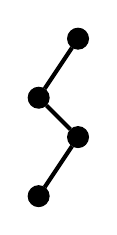
\begin{tikzpicture}
	\node (a) at (0.25cm,1cm) {};
	\node (b) at (-0.25cm,0.25cm) {};
	\node (c) at (0.25cm,-0.25cm) {};
	\node (d) at (-0.25cm,-1cm) {};
	\draw (a) edge (b); \draw (b) edge (c); \draw (c) edge (d);
\end{tikzpicture}
$\qquad$
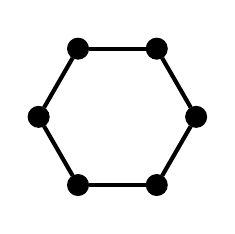
\begin{tikzpicture}
	\node (a) at (180:1cm) {};
	\node (b) at (120:1cm) {};
	\node (c) at (60:1cm) {};
	\node (d) at (0:1cm) {};
	\node (e) at (300:1cm) {};
	\node (f) at (240:1cm) {};
	\node [draw=none, fill=none] (1) at (0cm,-1cm) {};
	\node [draw=none, fill=none] (2) at (0cm,1cm) {};
	\draw (a) edge (b); \draw (b) edge (c); \draw (c) edge (d);
	\draw (d) edge (e); \draw (e) edge (f); \draw (f) edge (a);
\end{tikzpicture}\\
\hfill\\

\footnotesize{A length $4$ path, and a $6$-cycle.}
\end{center}
\end{frame}

\begin{frame}{Coloring}
A (vertex) \textbf{coloring} of a graph assigns a color to each vertex. A
$k$-coloring is a coloring that uses at most $k$ colors.\\
\hfill\\

\begin{center}
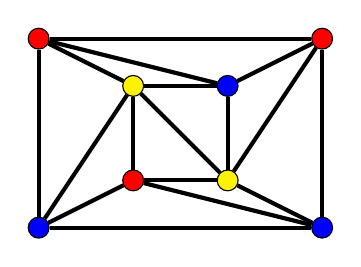
\begin{tikzpicture}[scale=0.6]
	\node (1) [fill=red] at (-3cm,2cm) {};
	\node (2) [fill=red] at (3cm,2cm) {};
	\node (3) [fill=blue] at (3cm,-2cm) {};
	\node (4) [fill=blue] at (-3cm,-2cm) {};
	\node (5) [fill=yellow] at (-1cm,1cm) {};
	\node (6) [fill=blue] at (1cm,1cm) {};
	\node (7) [fill=yellow] at (1cm,-1cm) {};
	\node (8) [fill=red] at (-1cm,-1cm) {};
	
	\draw (1) edge (2); \draw (2) edge (3); \draw (3) edge (4);
	\draw (4) edge (1);
	\draw (5) edge (6); \draw (6) edge (7); \draw (7) edge (8);
	\draw (8) edge (5);
	\draw (1) edge (5); \draw (2) edge (6); \draw (3) edge (7);
	\draw (4) edge (8);
	\draw (4) edge (5); \draw (1) edge (6); \draw (2) edge (7);
	\draw (3) edge (8); \draw (5) edge (7);
\end{tikzpicture}
$ \ $
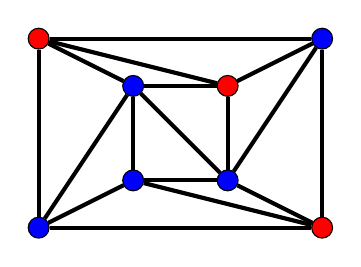
\begin{tikzpicture}[scale=0.6]
	\node (1) [fill=red] at (-3cm,2cm) {};
	\node (2) [fill=blue] at (3cm,2cm) {};
	\node (3) [fill=red] at (3cm,-2cm) {};
	\node (4) [fill=blue] at (-3cm,-2cm) {};
	\node (5) [fill=blue] at (-1cm,1cm) {};
	\node (6) [fill=red] at (1cm,1cm) {};
	\node (7) [fill=blue] at (1cm,-1cm) {};
	\node (8) [fill=blue] at (-1cm,-1cm) {};
	
	\draw (1) edge (2); \draw (2) edge (3); \draw (3) edge (4);
	\draw (4) edge (1);
	\draw (5) edge (6); \draw (6) edge (7); \draw (7) edge (8);
	\draw (8) edge (5);
	\draw (1) edge (5); \draw (2) edge (6); \draw (3) edge (7);
	\draw (4) edge (8);
	\draw (4) edge (5); \draw (1) edge (6); \draw (2) edge (7);
	\draw (3) edge (8); \draw (5) edge (7);
\end{tikzpicture}\\
\hfill\\
\footnotesize{Two different colorings.}
\end{center}
\end{frame}

\begin{frame}{Coloring}
The set of all vertices of a particular color is called a \textbf{color class}.\\
\hfill\\

\begin{center}
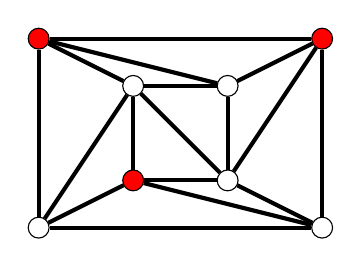
\begin{tikzpicture}[scale=0.6]
	\node (1) [fill=red] at (-3cm,2cm) {};
	\node (2) [fill=red] at (3cm,2cm) {};
	\node (3) [fill=blue, fill=none] at (3cm,-2cm) {};
	\node (4) [fill=blue, fill=none] at (-3cm,-2cm) {};
	\node (5) [fill=yellow, fill=none] at (-1cm,1cm) {};
	\node (6) [fill=blue, fill=none] at (1cm,1cm) {};
	\node (7) [fill=yellow, fill=none] at (1cm,-1cm) {};
	\node (8) [fill=red] at (-1cm,-1cm) {};
	
	\draw (1) edge (2); \draw (2) edge (3); \draw (3) edge (4);
	\draw (4) edge (1);
	\draw (5) edge (6); \draw (6) edge (7); \draw (7) edge (8);
	\draw (8) edge (5);
	\draw (1) edge (5); \draw (2) edge (6); \draw (3) edge (7);
	\draw (4) edge (8);
	\draw (4) edge (5); \draw (1) edge (6); \draw (2) edge (7);
	\draw (3) edge (8); \draw (5) edge (7);
\end{tikzpicture}
$ \ $
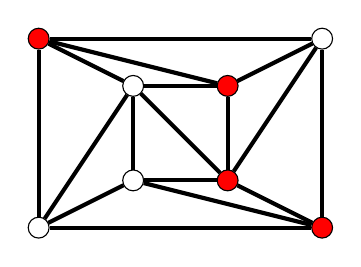
\begin{tikzpicture}[scale=0.6]
	\node (1) [fill=red] at (-3cm,2cm) {};
	\node (2) [fill=blue, fill=none] at (3cm,2cm) {};
	\node (3) [fill=red] at (3cm,-2cm) {};
	\node (4) [fill=blue, fill=none] at (-3cm,-2cm) {};
	\node (5) [fill=blue, fill=none] at (-1cm,1cm) {};
	\node (6) [fill=red] at (1cm,1cm) {};
	\node (7) [fill=red] at (1cm,-1cm) {};
	\node (8) [fill=blue, fill=none] at (-1cm,-1cm) {};
	
	\draw (1) edge (2); \draw (2) edge (3); \draw (3) edge (4);
	\draw (4) edge (1);
	\draw (5) edge (6); \draw (6) edge (7); \draw (7) edge (8);
	\draw (8) edge (5);
	\draw (1) edge (5); \draw (2) edge (6); \draw (3) edge (7);
	\draw (4) edge (8);
	\draw (4) edge (5); \draw (1) edge (6); \draw (2) edge (7);
	\draw (3) edge (8); \draw (5) edge (7);
\end{tikzpicture}\\
\hfill\\
\footnotesize{The color class of red in each graph.}
\end{center}
\end{frame}

\begin{frame}{Path coloring}
A \textbf{path coloring} is a coloring such that each color class induces a
collection of disjoint paths.\\
\hfill\\

\begin{center}
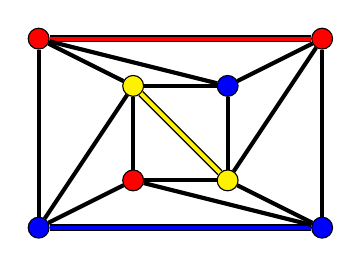
\begin{tikzpicture}[scale=0.6]
	\node (1) [fill=red] at (-3cm,2cm) {};
	\node (2) [fill=red] at (3cm,2cm) {};
	\node (3) [fill=blue] at (3cm,-2cm) {};
	\node (4) [fill=blue] at (-3cm,-2cm) {};
	\node (5) [fill=yellow] at (-1cm,1cm) {};
	\node (6) [fill=blue] at (1cm,1cm) {};
	\node (7) [fill=yellow] at (1cm,-1cm) {};
	\node (8) [fill=red] at (-1cm,-1cm) {};
	
	\draw (1) edge [line width=2.5pt] (2); \draw (3) edge [line width=2.5pt] (4);
	\draw (1) edge [color=red] (2); \draw (2) edge (3);
	\draw (3) edge [color=blue] (4); \draw (4) edge (1);
	\draw (5) edge (6); \draw (6) edge (7); \draw (7) edge (8);
	\draw (8) edge (5);
	\draw (1) edge (5); \draw (2) edge (6); \draw (3) edge (7);
	\draw (4) edge (8);
	\draw (4) edge (5); \draw (1) edge (6); \draw (2) edge (7);
	\draw (3) edge (8); \draw (5) edge [line width=2.5pt] (7);
	\draw (5) edge [color=yellow] (7);
\end{tikzpicture}
$ \ $
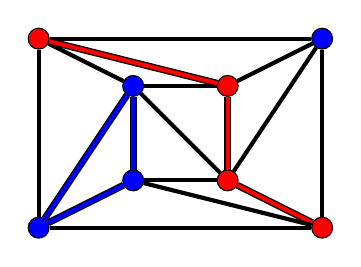
\begin{tikzpicture}[scale=0.6]
	\node (1) [fill=red] at (-3cm,2cm) {};
	\node (2) [fill=blue] at (3cm,2cm) {};
	\node (3) [fill=red] at (3cm,-2cm) {};
	\node (4) [fill=blue] at (-3cm,-2cm) {};
	\node (5) [fill=blue] at (-1cm,1cm) {};
	\node (6) [fill=red] at (1cm,1cm) {};
	\node (7) [fill=red] at (1cm,-1cm) {};
	\node (8) [fill=blue] at (-1cm,-1cm) {};
	
	\draw (1) edge [line width=2.5pt] (6); \draw (6) edge [line width=2.5pt] (7);
	\draw (3) edge [line width=2.5pt] (7); \draw (8) edge [line width=2.5pt] (5);
	\draw (4) edge [line width=2.5pt] (5); \draw (4) edge [line width=2.5pt] (8);
	\draw (1) edge (2); \draw (2) edge (3); \draw (3) edge (4);
	\draw (4) edge (1);
	\draw (5) edge (6); \draw (6) edge [color=red] (7); \draw (7) edge (8);
	\draw (8) edge [color=blue] (5);
	\draw (1) edge (5); \draw (2) edge (6); \draw (3) edge [color=red] (7);
	\draw (4) edge [color=blue] (8);
	\draw (4) edge [color=blue] (5); \draw (1) edge [color=red] (6); \draw (2) edge (7);
	\draw (3) edge (8); \draw (5) edge (7);
\end{tikzpicture}\\
\hfill\\
\footnotesize{A path $3$-coloring and a $2$-coloring that is not a path
coloring.}
\end{center}
\end{frame}

\begin{frame}{Poh}
\begin{thm}[Poh, 1990]
All planar graphs admit a path $3$-coloring.
\end{thm}

In his proof Poh described a constructive procedure to produce such a coloring.
We will describe an efficient implementation of Poh's algorithm.
\end{frame}

\section{Graph representations}

\begin{frame}{Representing graphs}
In order to work with graphs on computers we require an efficient data
structure to represent a graph.

Suppose $G$ is a graph with $n$ vertices and $m$ edges. We will assume the
vertices of $G$ are the integers $1,2,\ldots,n$.

The input size will always be the number of vertices $n$. However, for plane
graphs $\mathcal{O}(m)=\mathcal{O}(n)$, so it is equivalent to take the input
size to be the number of edges.
\end{frame}

\begin{frame}{Adjacency lists}
For each vertex we define a linked list known as an \textbf{adjacency list}
containing its neighbors. The full graph is then represented by a size $n$ array
$\text{Adj}$ such that each vertex $v$ has adjacency list $\text{Adj}[v]$.\\

\begin{center}
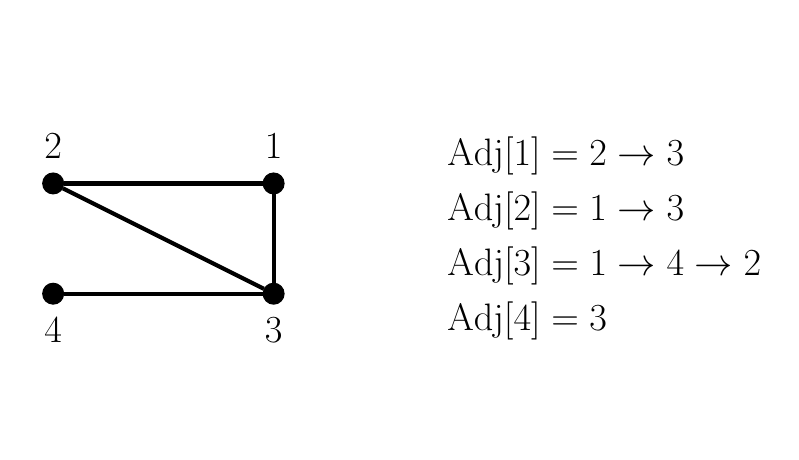
\begin{tikzpicture}[scale=.7]
  \node (a) [label=above:$1$] at (2cm,1cm) {};
  \node (b) [label=above:$2$]  at (-2cm,1cm) {};
  \node (c) [label=below:$3$]  at (2cm,-1cm) {};
  \node (d) [label=below:$4$]  at (-2cm,-1cm) {};
  \node [draw=none, fill=none] (1) at (7.3cm,1.5cm) {$\text{Adj}[1]=2\rightarrow 3$};
  \node [draw=none, fill=none] (2) at (7.3cm,0.5cm) {$\text{Adj}[2]=1\rightarrow 3$};
  \node [draw=none, fill=none] (3) at (8cm,-0.5cm) {$\text{Adj}[3]=1\rightarrow 4\rightarrow 2$};
  \node [draw=none, fill=none] (4) at (6.6cm,-1.5cm) {$\text{Adj}[4]=3$};
  \draw (a) edge (c); \draw (c) edge (d);
  \draw (a) edge (b); \draw (b) edge (c);
\end{tikzpicture}
\end{center}
\end{frame}

\begin{frame}{Adjacency lists}
Adjacency list representations may simultaneously store a rotation scheme for
a plane graph by ordering the neighbors in each list.

\begin{center}
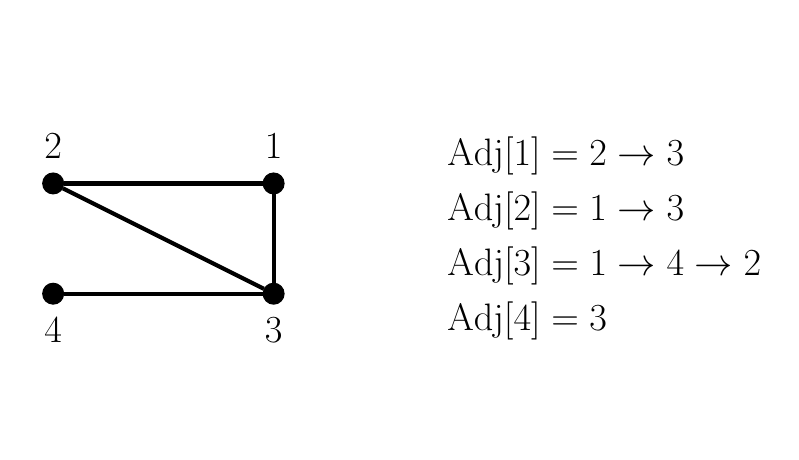
\begin{tikzpicture}[scale=.7]
  \node (a) [label=above:$1$] at (2cm,1cm) {};
  \node (b) [label=above:$2$]  at (-2cm,1cm) {};
  \node (c) [label=below:$3$]  at (2cm,-1cm) {};
  \node (d) [label=below:$4$]  at (-2cm,-1cm) {};
  \node [draw=none, fill=none] (1) at (7.3cm,1.5cm) {$\text{Adj}[1]=2\rightarrow 3$};
  \node [draw=none, fill=none] (2) at (7.3cm,0.5cm) {$\text{Adj}[2]=1\rightarrow 3$};
  \node [draw=none, fill=none] (3) at (8cm,-0.5cm) {$\text{Adj}[3]=1\rightarrow 4\rightarrow 2$};
  \node [draw=none, fill=none] (4) at (6.6cm,-1.5cm) {$\text{Adj}[4]=3$};
  \draw (a) edge (c); \draw (c) edge (d);
  \draw (a) edge (b); \draw (b) edge (c);
\end{tikzpicture}
\end{center}
\end{frame}

\begin{frame}{Triangulations}
Given an arbitrary planar graph with an adjacency list representation, linear
time algorithms exist to embed it in the plane, i.e. order it's adjacency lists
such that they correspond to a drawing of the graph with no edge crossings.

Moreover, given a plane graph, linear time algorithms exist to add edges until
the graph is triangulated.
\end{frame}

\begin{frame}{Vertex properties}
\begin{ida}<1->
We often wish to track various properties about the vertices of a graph,
such as what color they have received, or whether they are in a particular
subgraph.
\end{ida}

\begin{imp}<2->
Properties will be represented by constructing a size $n$ array indexed by
vertices. Thus accessing a vertex property will be a basic operation.
\end{imp}

\begin{exm}<3->
An adjacency list is a vertex property.
\end{exm}
\end{frame}

\begin{frame}{Vertex marking}
We will often use an integer vertex property called a mark.

To represent a path or cycle we mark all vertices on the path or cycle with a
unique integer identifying the path.

To perform a breadth first search we mark vertices that have already been
visited.
\end{frame}

\begin{frame}{Cycles and plane graphs}
Given a cycle in a plane graph we are guaranteed no interior vertices are
connected with exterior vertices. Therefore by marking a cycle in our graph we
simultaneously represent a subgraph.\\
\hfill\\

\begin{center}
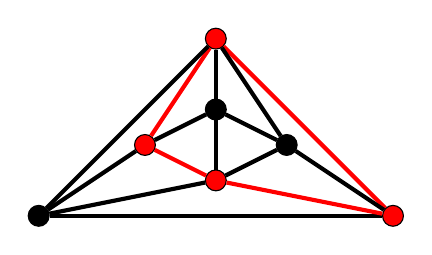
\begin{tikzpicture}[scale=.45]
  \node (0) at (0cm, 0cm) {};
  \node (1) at (7cm, 2cm) {};
  \node (2) [fill=red] at (10cm, 0cm) {};
  \node (3) [fill=red] at (3cm, 2cm) {};
  \node (4) [fill=red] at (5cm, 5cm) {};
  \node (5) [fill=red] at (5cm, 1cm) {};
  \node (6) at (5cm, 3cm) {};
  
  \draw (0) edge (2); \draw (2) edge [color=red] (5); \draw (0) edge (5);
  \draw (3) edge (0); \draw (4) edge (6); \draw (5) edge (1);
  \draw (3) edge (6); \draw (2) edge [color=red] (4); \draw (6) edge (1);
  \draw (4) edge [color=red] (3); \draw (4) edge (0); \draw (1) edge (4);
  \draw (1) edge (2); \draw (5) edge [color=red] (3); \draw (5) edge (6);
\end{tikzpicture}
$ \ $
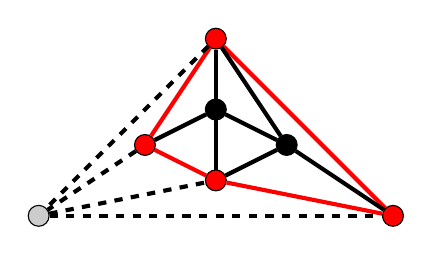
\begin{tikzpicture}[scale=.45]
  \node (0) [fill opacity=0.2] at (0cm, 0cm) {};
  \node (1) at (7cm, 2cm) {};
  \node (2) [fill=red] at (10cm, 0cm) {};
  \node (3) [fill=red] at (3cm, 2cm) {};
  \node (4) [fill=red] at (5cm, 5cm) {};
  \node (5) [fill=red] at (5cm, 1cm) {};
  \node (6) at (5cm, 3cm) {};
  
  \draw (0) edge [dashed] (2); \draw (2) edge [color=red] (5); \draw (0) edge [dashed] (5);
  \draw (3) edge [dashed] (0); \draw (4) edge (6); \draw (5) edge (1);
  \draw (3) edge (6); \draw (2) edge [color=red] (4); \draw (6) edge (1);
  \draw (4) edge [color=red] (3); \draw (4) edge [dashed] (0); \draw (1) edge (4);
  \draw (1) edge (2); \draw (5) edge [color=red] (3); \draw (5) edge (6);
\end{tikzpicture}\\
\hfill\\
\footnotesize{A cycle in a triangulated graph.}
\end{center}
\end{frame}

\section{Path $3$-coloring plane graphs}

\begin{frame}{Poh's algorithm}
\textbf{Input:} A weakly triangulated plane graph $G$ such that it's outer face
is a cycle $C$, and a $2$-coloring of $C$ such that each color class induces
a path, denoted $P$ and $Q$ respectively.

\textbf{Output:} An extension of the $2$-coloring of $C$ to a path $3$-coloring
of $G$ such that no vertex in $C$ receives a same color neighbor in $G-C$.

\begin{center}
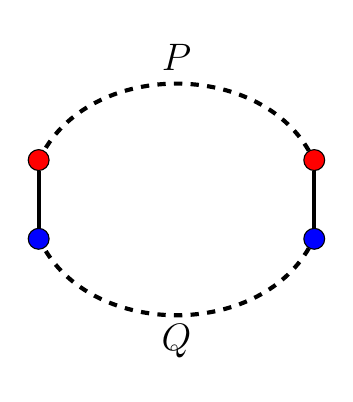
\begin{tikzpicture}
  \node (p0) [fill=red] at (1.5cm, 0.5cm) {};
  \node (pn) [fill=red] at (-2cm, 0.5cm) {};
  \node (q0) [fill=blue] at (1.5cm, -0.5cm) {};
  \node (qn) [fill=blue] at (-2cm, -0.5cm) {};
  \node (null) [draw=none, fill=none] at (270:1.5cm) {};
  
  \node (P) [draw=none, fill=none] at (-0.25cm, 1.8cm) {$P$};
  \node (Q) [draw=none, fill=none] at (-0.25cm, -1.8cm) {$Q$};
  
  \draw (p0) edge [bend right=60] (pn) [dashed];
  \draw (q0) edge [bend left=60] (qn) [dashed];
  \draw (p0) edge (q0);
  \draw (pn) edge (qn);
\end{tikzpicture}
\end{center}
\end{frame}

\begin{frame}{Poh's algorithm}
\begin{cse}[1]
If there exists an edge between $P$ and $Q$ that is not in $C$ we may apply
Poh's algorithm to separately path $3$-color the interior of the cycles $C_1$
and $C_2$ seen below.
\end{cse}

\begin{center}
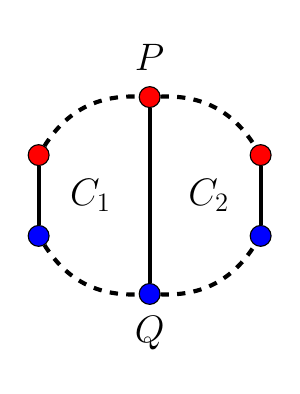
\begin{tikzpicture}
  \node (p0) [fill=red] at (160:1.5cm) {};
  \node (p1) [fill=red] at (90:1.25cm) {};
  \node (pn) [fill=red] at (20:1.5cm) {};
  \node (q0) [fill=blue] at (200:1.5cm) {};
  \node (q1) [fill=blue] at (270:1.25cm) {};
  \node (qn) [fill=blue] at (340:1.5cm) {};
  \node (null) [fill=none,draw=none] at (270:1.75cm) {};
  
  \node (C1) [draw=none, fill=none] at (180:0.75cm) {$C_1$};
  \node (C2) [draw=none, fill=none] at (0:0.75cm) {$C_2$};
  
  \node (P) [draw=none, fill=none] at (90:1.75cm) {$P$};
  \node (Q) [draw=none, fill=none] at (270:1.75cm) {$Q$};
  
  \draw (p0) edge [bend left] (p1) [dashed];
  \draw (p1) edge [bend left] (pn) [dashed];
  \draw (q0) edge [bend right] (q1) [dashed];
  \draw (q1) edge [bend right] (qn) [dashed];
  \draw (p0) edge (q0);
  \draw (pn) edge (qn);
  \draw (p1) edge (q1);
\end{tikzpicture}
\end{center}
\end{frame}

\begin{frame}{Poh's algorithm}
\begin{cse}[2]
If no such edge exists and there are vertices left to color then we find
the shortest path $T$ through the interior. We may then color $T$ with the
remaining color and apply Poh's algorithm to separately color the interior
of the cycles $C_1$ and $C_2$ seen below.
\end{cse}

\begin{center}
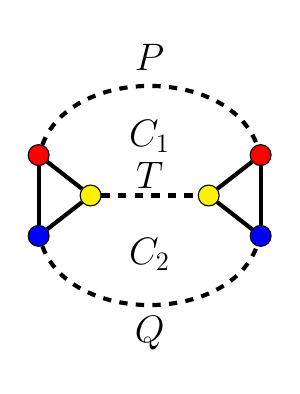
\begin{tikzpicture}
  \node (p0) [fill=red] at (160:1.5cm) {};
  \node (pn) [fill=red] at (20:1.5cm) {};
  \node (q0) [fill=blue] at (200:1.5cm) {};
  \node (qn) [fill=blue] at (340:1.5cm) {};
  \node (t0) [fill=yellow] at (180:0.75cm) {};
  \node (t1) [fill=yellow] at (0:0.75cm) {};
  \node (null) [draw=none, fill=none] at (270:1.75cm) {};
  
  \node (C1) [draw=none, fill=none] at (90:0.75cm) {$C_1$};
  \node (C2) [draw=none, fill=none] at (270:0.75cm) {$C_2$};
  
  \node (P) [draw=none, fill=none] at (90:1.75cm) {$P$};
  \node (Q) [draw=none, fill=none] at (270:1.75cm) {$Q$};
  \node (T) [draw=none, fill=none] at (90:0.25cm) {$T$};
  
  \draw (p0) edge [bend left=70] (pn) [dashed];
  \draw (q0) edge [bend right=70] (qn) [dashed];
  \draw (p0) edge (q0);
  \draw (pn) edge (qn);
  \draw (p0) edge (t0);
  \draw (q0) edge (t0);
  \draw (pn) edge (t1);
  \draw (qn) edge (t1);
  \draw (t0) edge (t1) [dashed];
\end{tikzpicture}
\end{center}
\end{frame}

\begin{frame}{Procedure to path $3$-color a planar graph}
Given an arbitrary plane graph we may add edges until it is triangulated.

By path $2$-coloring the outer triangle of the triangulated graph we may then
apply Poh's algorithm to produce a path $3$-coloring.

The resulting coloring is also a $3$-coloring of the original graph, with the
additional ``triangulation edges" removed.
\end{frame}

\begin{frame}{Implementing Poh's algorithm}
\textbf{Input:} A triangulated graph, and the first and last vertex of two marked paths
$P=p_1p_2\ldots p_k$ and $Q=q_1q_2\ldots q_l$ that satisfy the requirements
of Poh's algorithm.

\textbf{Output:} A path $3$-coloring of the interior of the cycle formed by $P$
and $Q$ such that none of the vertices in $P$ or $Q$ receive a new same color
neighbor.

\begin{center}
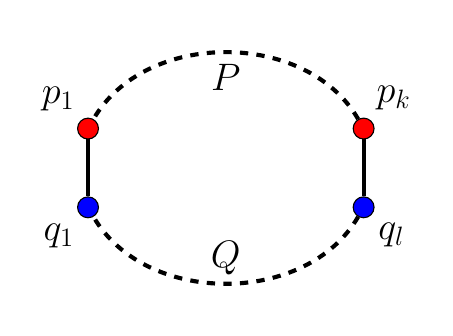
\begin{tikzpicture}
  \node (p0) [label=above right:$p_k$, fill=red] at (1.5cm, 0.5cm) {};
  \node (pn) [label=above left:$p_1$, fill=red] at (-2cm, 0.5cm) {};
  \node (q0) [label=below right:$q_l$, fill=blue] at (1.5cm, -0.5cm) {};
  \node (qn) [label=below left:$q_1$, fill=blue] at (-2cm, -0.5cm) {};
  \node (null) [draw=none, fill=none] at (270:1.5cm) {};
  
  \node (P) [draw=none, fill=none] at (-0.25cm, 1.15cm) {$P$};
  \node (Q) [draw=none, fill=none] at (-0.25cm, -1.15cm) {$Q$};
  
  \draw (p0) edge [bend right=60] (pn) [dashed];
  \draw (q0) edge [bend left=60] (qn) [dashed];
  \draw (p0) edge (q0);
  \draw (pn) edge (qn);
\end{tikzpicture}
\end{center}
\end{frame}

\begin{frame}{Implementing Poh's algorithm}
We begin by locating $q_1$ in $\text{Adj}[p_1]$. Let $u$ be the
vertex clockwise from $q_1$ in $\text{Adj}[p_1]$. Note the cycle $p_1q_1u$ is
a triangle face.

If $u$ is in $P$ we apply the algorithm to $P-p_1$ and $Q$. Similarly, if $u$ is
in $Q$ we apply the algorithm to $P$ and $Q-q_1$.

\begin{center}
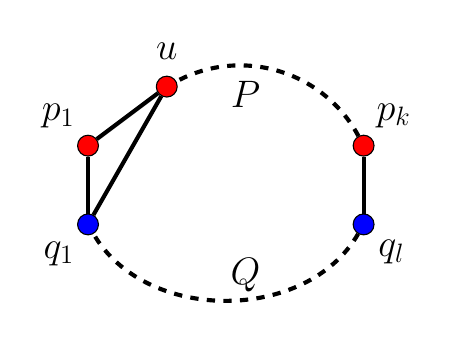
\begin{tikzpicture}
  \node (p0) [label=above right:$p_k$, fill=red] at (1.5cm, 0.5cm) {};
  \node (pn) [label=above left:$p_1$, fill=red] at (-2cm, 0.5cm) {};
  \node (q0) [label=below right:$q_l$, fill=blue] at (1.5cm, -0.5cm) {};
  \node (qn) [label=below left:$q_1$, fill=blue] at (-2cm, -0.5cm) {};
  \node (t) [label=above:$u$, fill=red] at (-1cm, 1.25cm) {};
  \node (null) [draw=none, fill=none] at (270:1.5cm) {};
  
  \node (P) [draw=none, fill=none] at (0cm, 1.15cm) {$P$};
  \node (Q) [draw=none, fill=none] at (0cm, -1.15cm) {$Q$};
  
  \draw (t) edge (pn);
  \draw (qn) edge (t);
  \draw (p0) edge [bend right=45] (t) [dashed];
  \draw (q0) edge [bend left=60] (qn) [dashed];
  \draw (p0) edge (q0);
  \draw (pn) edge (qn);
\end{tikzpicture}
\end{center}
\end{frame}

\begin{frame}{Implementing Poh's algorithm}
Otherwise, $u$ is an interior vertex. Perform
a breadth first search from $u$ through the interior vertices until we find
a vertex $v$ with a neighbor in $Q$ immediately clockwise from a neighbor in
$P$. We may then backtrack along the search to color the path $T$.

\begin{center}
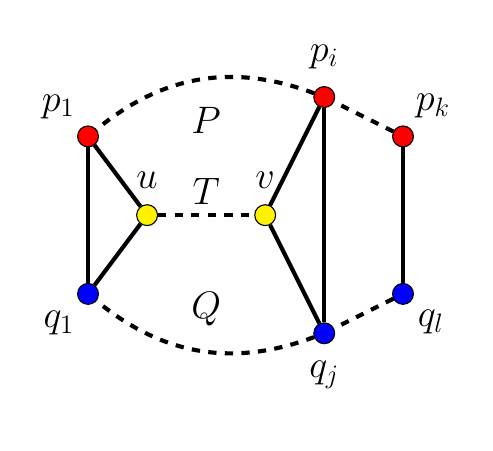
\begin{tikzpicture}
  \node (p0) [fill=red, label=above right:{$p_k$}] at (2cm, 1cm) {};
  \node (pn) [label=above left:$p_1$, fill=red] at (-2cm, 1cm) {};
  \node (q0) [fill=blue, label=below right:{$q_l$}] at (2cm, -1cm) {};
  \node (qn) [label=below left:$q_1$, fill=blue] at (-2cm, -1cm) {};
  \node (t0) [label=above:$v$, fill=yellow] at (0.25cm, 0cm) {};
  \node (t1) [label=above:$u$, fill=yellow] at (-1.25cm, 0cm) {};
  \node (pi) [fill=red,  label=above:{$p_i$}] at (1cm, 1.5cm) {};
  \node (qj) [fill=blue, label=below:{$q_j$}] at (1cm, -1.5cm) {};
  
  \node (T) [draw=none, fill=none] at (-0.5cm, 0.3cm) {$T$};
  \node (P) [draw=none, fill=none] at (-0.5cm, 1.2cm) {$P$};
  \node (Q) [draw=none, fill=none] at (-0.5cm, -1.2cm) {$Q$};
  
  \node (null) [draw=none, fill=none] at (270:2.5cm) {};
  
  \draw (p0) edge (pi) [dashed];
  \draw (pi) edge [bend right] (pn) [dashed];
  \draw (q0) edge (qj) [dashed];
  \draw (qj) edge [bend left] (qn) [dashed];
  \draw (p0) edge (q0);
  \draw (pn) edge (qn);
  \draw (pi) edge (qj);
  \draw (pn) edge (t1);
  \draw (qn) edge (t1);

  \draw (t1) edge (t0) [dashed];
  \draw (pi) edge (t0);
  \draw (qj) edge (t0);
\end{tikzpicture}
\end{center}
\end{frame}

\begin{frame}{Implementing Poh's algorithm}
\begin{center}
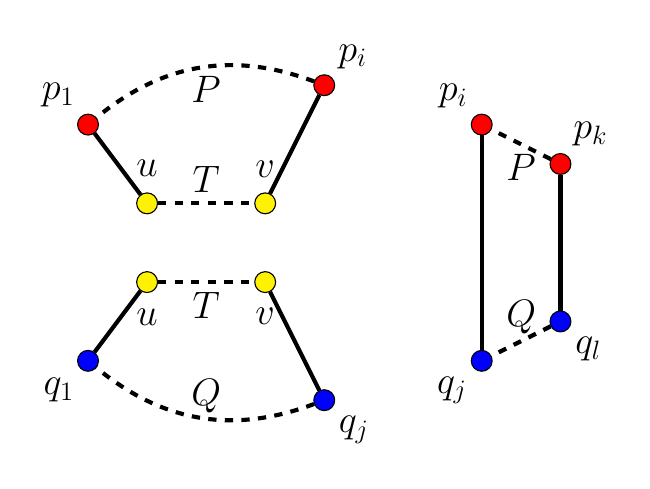
\begin{tikzpicture}
  \node (p0) [fill=red, label=above right:{$p_k$}] at (4cm, 1cm) {};
  \node (q0) [fill=blue, label=below right:{$q_l$}] at (4cm, -1cm) {};
  \node (pi) [fill=red, label=above left:{$p_i$}] at (3cm, 1.5cm) {};
  \node (qj) [fill=blue, label=below left:{$q_j$}] at (3cm, -1.5cm) {};
  
  \node (pi_1) [fill=red, label=above right:$p_i$] at (1cm, 2cm) {};
  \node (pn) [fill=red, label=above left:$p_1$] at (-2cm, 1.5cm) {};
  \node (t0) [label=above:$v$, fill=yellow] at (0.25cm, 0.5cm) {};
  \node (t1) [label=above:$u$, fill=yellow] at (-1.25cm, 0.5cm) {};
  
  \node (T) [draw=none, fill=none] at (-0.5cm, 0.8cm) {$T$};
  \node (T1) [draw=none, fill=none] at (-0.5cm, -0.8cm) {$T$};
  \node (P) [draw=none, fill=none] at (-0.5cm, 1.95cm) {$P$};
  \node (P1) [draw=none, fill=none] at (3.5cm, 0.95cm) {$P$};
  \node (Q) [draw=none, fill=none] at (-0.5cm, -1.95cm) {$Q$};
  \node (Q1) [draw=none, fill=none] at (3.5cm, -0.95cm) {$Q$};
  
  \node (qj_1) [fill=blue,  label=below right:$q_j$] at (1cm, -2cm) {};
  \node (qn) [label=below left:$q_1$, fill=blue] at (-2cm, -1.5cm) {};
  \node (t0_1) [label=below:$v$, fill=yellow] at (0.25cm, -0.5cm) {};
  \node (t1_1) [label=below:$u$, fill=yellow] at (-1.25cm, -0.5cm) {};
  \node (null) [draw=none, fill=none] at (270:2.5cm) {};
  
  \draw (p0) edge (pi) [dashed];
  \draw (pi_1) edge [bend right] (pn) [dashed];
  \draw (q0) edge (qj) [dashed];
  \draw (qj_1) edge [bend left] (qn) [dashed];
  \draw (p0) edge (q0);
  \draw (pi) edge (qj);
  \draw (pn) edge (t1);
  \draw (qn) edge (t1_1);
  \draw (t1) edge (t0) [dashed];
  \draw (t1_1) edge (t0_1) [dashed];
  \draw (pi_1) edge (t0);
  \draw (qj_1) edge (t0_1);
\end{tikzpicture}
\end{center}
\end{frame}

\begin{frame}{Poh coloring example}
\begin{center}
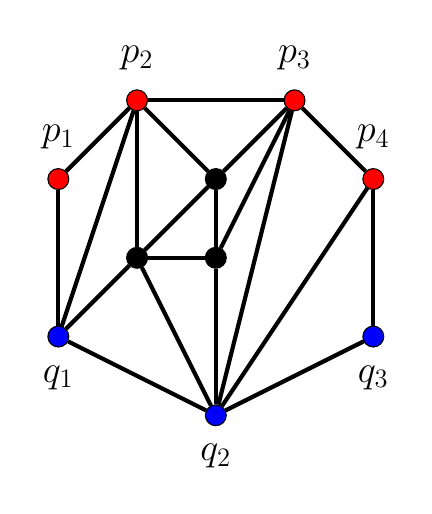
\begin{tikzpicture}
  \node (1) [fill=red, label=above:$p_1$] at (-2cm, 1cm) {};
  \node (2) [fill=red, label=above:$p_2$] at (-1cm, 2cm) {};
  \node (3) [fill=red, label=above:$p_3$] at (1cm, 2cm) {};
  \node (4) [fill=red, label=above:$p_4$] at (2cm, 1cm) {};
  \node (5) [fill=blue, label=below:$q_3$] at (2cm, -1cm) {};
  \node (6) [fill=blue, label=below:$q_2$] at (0cm, -2cm) {};
  \node (7) [fill=blue, label=below:$q_1$] at (-2cm, -1cm) {};
  \node (8) at (-1cm, 0cm) {};
  \node (9) at (0cm, 1cm) {};
  \node (10) at (0cm, 0cm) {};
  
  \draw (1) edge (2); \draw (2) edge (3); \draw (3) edge (4);
  \draw (4) edge (5); \draw (5) edge (6); \draw (6) edge (7);
  \draw (7) edge (1); \draw (2) edge (7); \draw (2) edge (8);
  \draw (2) edge (9); \draw (3) edge (9); \draw (3) edge (6);
  \draw (4) edge (6); \draw (6) edge (8); \draw (6) edge (10);
  \draw (7) edge (8); \draw (8) edge (9); \draw (8) edge (10);
  \draw (9) edge (10); \draw (10) edge (3);
\end{tikzpicture}
\end{center}
\end{frame}

\begin{frame}{Poh coloring example}
\begin{center}
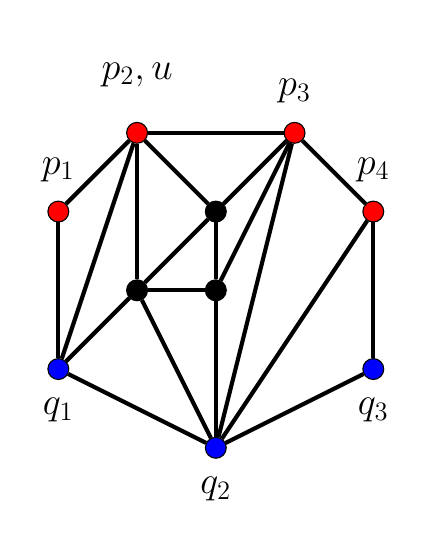
\begin{tikzpicture}
  \node (1) [fill=red, label=above:$p_1$] at (-2cm, 1cm) {};
  \node (2) [fill=red, label=above:{$p_2,u$}] at (-1cm, 2cm) {};
  \node (3) [fill=red, label=above:$p_3$] at (1cm, 2cm) {};
  \node (4) [fill=red, label=above:$p_4$] at (2cm, 1cm) {};
  \node (5) [fill=blue, label=below:$q_3$] at (2cm, -1cm) {};
  \node (6) [fill=blue, label=below:$q_2$] at (0cm, -2cm) {};
  \node (7) [fill=blue, label=below:$q_1$] at (-2cm, -1cm) {};
  \node (8) at (-1cm, 0cm) {};
  \node (9) at (0cm, 1cm) {};
  \node (10) at (0cm, 0cm) {};
  
  \draw (1) edge (2); \draw (2) edge (3); \draw (3) edge (4);
  \draw (4) edge (5); \draw (5) edge (6); \draw (6) edge (7);
  \draw (7) edge (1); \draw (2) edge (7); \draw (2) edge (8);
  \draw (2) edge (9); \draw (3) edge (9); \draw (3) edge (6);
  \draw (4) edge (6); \draw (6) edge (8); \draw (6) edge (10);
  \draw (7) edge (8); \draw (8) edge (9); \draw (8) edge (10);
  \draw (9) edge (10); \draw (10) edge (3);
\end{tikzpicture}
\end{center}
\end{frame}

\begin{frame}{Poh coloring example}
\begin{center}
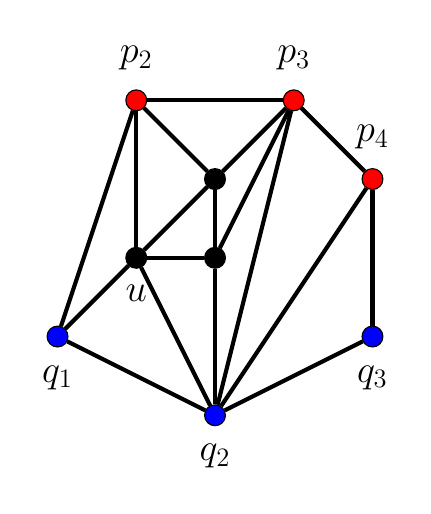
\begin{tikzpicture}
  \node (1) [draw=none, fill=none] at (-2cm, 1cm) {};
  \node (2) [fill=red, label=above:$p_2$] at (-1cm, 2cm) {};
  \node (3) [fill=red, label=above:$p_3$] at (1cm, 2cm) {};
  \node (4) [fill=red, label=above:$p_4$] at (2cm, 1cm) {};
  \node (5) [fill=blue, label=below:$q_3$] at (2cm, -1cm) {};
  \node (6) [fill=blue, label=below:$q_2$] at (0cm, -2cm) {};
  \node (7) [fill=blue, label=below:$q_1$] at (-2cm, -1cm) {};
  \node (8) [label=below:$u$] at (-1cm, 0cm) {};
  \node (9) at (0cm, 1cm) {};
  \node (10) at (0cm, 0cm) {};
  
  \draw (2) edge (3); \draw (3) edge (4);
  \draw (4) edge (5); \draw (5) edge (6); \draw (6) edge (7);
  \draw (2) edge (7); \draw (2) edge (8);
  \draw (2) edge (9); \draw (3) edge (9); \draw (3) edge (6);
  \draw (4) edge (6); \draw (6) edge (8); \draw (6) edge (10);
  \draw (7) edge (8); \draw (8) edge (9); \draw (8) edge (10);
  \draw (9) edge (10); \draw (10) edge (3);
\end{tikzpicture}
\end{center}
\end{frame}

\begin{frame}{Poh coloring example}
\begin{center}
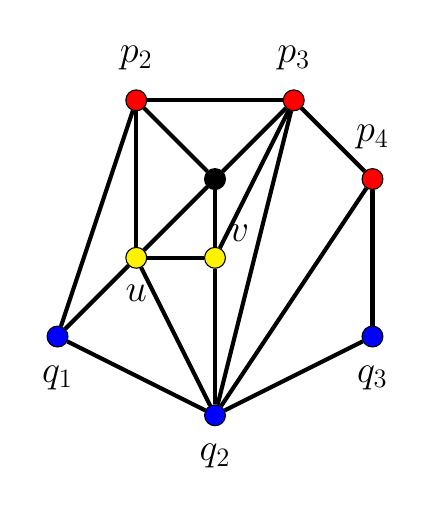
\begin{tikzpicture}
  \node (1) [draw=none, fill=none] at (-2cm, 1cm) {};
  \node (2) [fill=red, label=above:$p_2$] at (-1cm, 2cm) {};
  \node (3) [fill=red, label=above:$p_3$] at (1cm, 2cm) {};
  \node (4) [fill=red, label=above:$p_4$] at (2cm, 1cm) {};
  \node (5) [fill=blue, label=below:$q_3$] at (2cm, -1cm) {};
  \node (6) [fill=blue, label=below:$q_2$] at (0cm, -2cm) {};
  \node (7) [fill=blue, label=below:$q_1$] at (-2cm, -1cm) {};
  \node (8) [fill=yellow, label=below:$u$] at (-1cm, 0cm) {};
  \node (9) at (0cm, 1cm) {};
  \node (10) [fill=yellow, label=above right:$v$] at (0cm, 0cm) {};
  
  \draw (2) edge (3); \draw (3) edge (4);
  \draw (4) edge (5); \draw (5) edge (6); \draw (6) edge (7);
  \draw (2) edge (7); \draw (2) edge (8);
  \draw (2) edge (9); \draw (3) edge (9); \draw (3) edge (6);
  \draw (4) edge (6); \draw (6) edge (8); \draw (6) edge (10);
  \draw (7) edge (8); \draw (8) edge (9); \draw (8) edge (10);
  \draw (9) edge (10); \draw (10) edge (3);
\end{tikzpicture}
\end{center}
\end{frame}

\begin{frame}{Poh coloring example}
\begin{center}
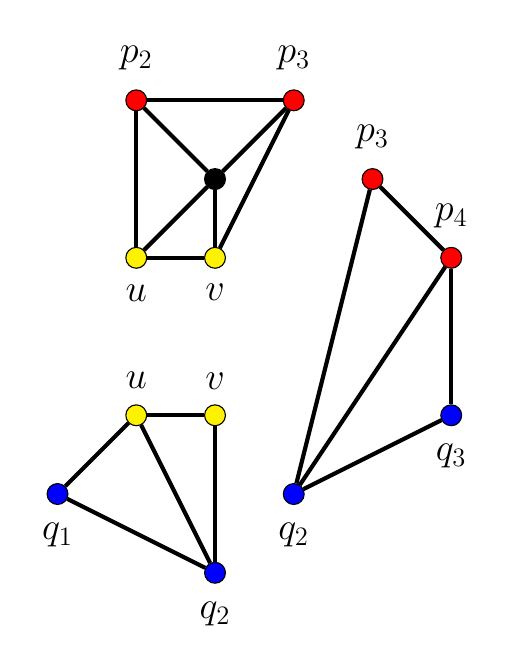
\begin{tikzpicture}
  \node (1) [draw=none, fill=none] at (-2cm, 1cm) {};
  
  \node (2) [fill=red, label=above:$p_2$] at (-1cm, 3cm) {};
  \node (3) [fill=red, label=above:$p_3$] at (1cm, 3cm) {};
  \node (8) [fill=yellow, label=below:$u$] at (-1cm, 1cm) {};
  \node (9) at (0cm, 2cm) {};
  \node (10) [fill=yellow, label=below:$v$] at (0cm, 1cm) {};
  
  \node (3c) [fill=red, label=above:$p_3$] at (2cm, 2cm) {};
  \node (4) [fill=red, label=above:$p_4$] at (3cm, 1cm) {};
  \node (5) [fill=blue, label=below:$q_3$] at (3cm, -1cm) {};
  \node (6) [fill=blue, label=below:$q_2$] at (1cm, -2cm) {};
  
  \node (6p) [fill=blue, label=below:$q_2$] at (0cm, -3cm) {};
  \node (7) [fill=blue, label=below:$q_1$] at (-2cm, -2cm) {};
  \node (8p) [fill=yellow, label=above:$u$] at (-1cm, -1cm) {};
  \node (10p) [fill=yellow, label=above:$v$] at (0cm, -1cm) {};
  
  \draw (2) edge (3); \draw (3c) edge (4);
  \draw (4) edge (5); \draw (5) edge (6); \draw (6p) edge (7);
  \draw (2) edge (8);
  \draw (2) edge (9); \draw (3) edge (9); \draw (3c) edge (6);
  \draw (4) edge (6); \draw (6p) edge (8p); \draw (6p) edge (10p);
  \draw (7) edge (8p); \draw (8) edge (9); \draw (8) edge (10);
  \draw (8p) edge (10p); \draw (9) edge (10); \draw (10) edge (3);
\end{tikzpicture}
\end{center}
\end{frame}

\begin{frame}{Poh time complexity}
Poh's algorithm potentially performs a breadth first in each call. Unfortunately
this results in a worst case running time that is not linear.

However, another way to find an induced path through the cycle is walking along
the inside one of the paths $P$ or $Q$. Using this method produces a similar
algorithm that runs in linear time.
\end{frame}

\section{Path $3$-list-coloring plane graphs}

\begin{frame}{Path $3$-list-coloring}
Suppose $L$ maps each vertex of a graph $G$ to a list of colors. Then a
\textbf{path list-coloring} of $G$ from $L$ is a path coloring such that each
vertex $v$ receives a color from $L(v)$.

\begin{thm}[Hartman, 1997]
All planar graphs admit a path list coloring if each vertex is assigned a list
of at least $3$ colors.
\end{thm}

The proof provides a constructive algorithm to produce a such a coloring.

Independently, around the same time Skrekovski proved a slightly weaker result
using the same coloring procedure.

We will describe Hartman and Skrekovski's coloring algorithm, and then
describe how it may be implemented in linear time.
\end{frame}


\begin{frame}{Hartman-Skrekovski list-coloring}
\textbf{Input:} A weakly triangulated plane graph $G$ whose outer face is a
cycle $C$, and a pair of vertices $x,y$ in $C$. Also, a list assignment $L$
such that $x$, $y$ receive at least $1$ color, other vertices in $C$ receive
at least $2$ colors, and interior vertices receive at least $3$ colors.

\textbf{Output:} A path list-coloring of $G$ from $L$.
\end{frame}

\begin{frame}{Hartman-Skrekovski list-coloring}
\begin{center}
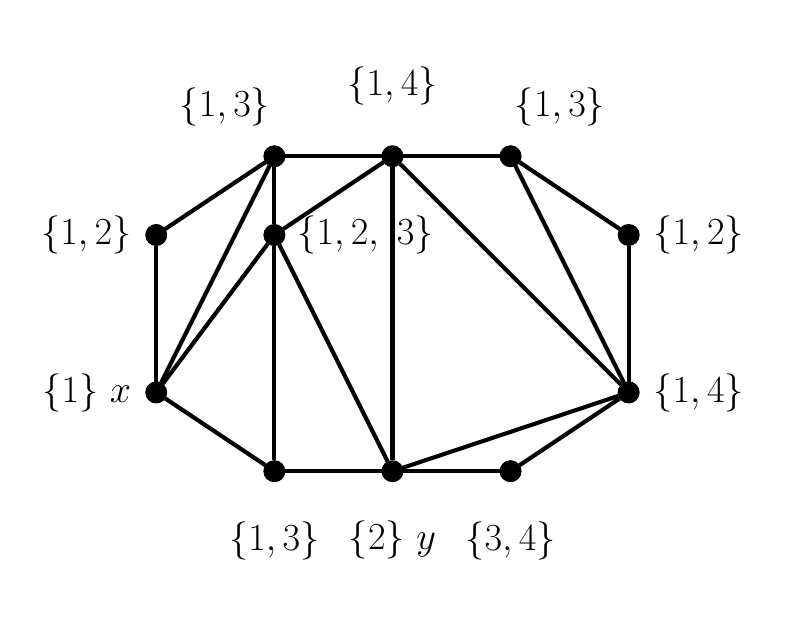
\begin{tikzpicture}
	\node (1) [label=left:{$\{1,2\}$}] at (-3.0cm, 1.0cm) {};
	\node (2) [label=above left:{$\{1,3\}$}] at (-1.5cm, 2.0cm) {};
	\node (3) [label=above:{$\{1,4\}$}] at (0.0cm, 2.0cm) {};
	\node (4) [label=above right:{$\{1,3\}$}] at (1.5cm, 2.0cm) {};
	\node (5) [label=right:{$\{1,2\}$}] at (3.0cm, 1.0cm) {};
	\node (6) [label=right:{$\{1,4\}$}] at (3.0cm, -1.0cm) {};
	\node (7) [label=below:{$\{3,4\}$}] at (1.5cm, -2.0cm) {};
	\node (8) [label=below:{$\{2\} \ y$}] at (0.0cm, -2.0cm) {};
	\node (9) [label=below:{$\{1,3\}$}] at (-1.5cm, -2.0cm) {};
	\node (10) [label=left:{$\{1\} \ x$}] at (-3.0cm, -1.0cm) {};
	\node (11) [label=right:{$\{1,2, \ 3\}$}] at (-1.5cm, 1.0cm) {};
	
	\draw (1) edge (2); \draw (2) edge (3); \draw (3) edge (4);
	\draw (4) edge (5); \draw (5) edge (6); \draw (6) edge (7);
	\draw (7) edge (8); \draw (8) edge (9); \draw (9) edge (10);
	\draw (10) edge (1);
	
	\draw (2) edge (11); \draw (3) edge (11); \draw (3) edge (6);
	\draw (4) edge (6); \draw (3) edge (8); \draw (6) edge (8);
	\draw (8) edge (11); \draw (9) edge (11); \draw (10) edge (11);
	\draw (10) edge (2);
\end{tikzpicture}
\end{center}
\end{frame}

\begin{frame}{Hartman-Skrekovski list-coloring}
Select a color $c$ from $L(x)$. We will now color an induced path with $c$ as
far as possible clockwise along $C$ towards $y$.

\textbf{Procedure:}

Initialize the path $P$ to contain the single vertex $x$. 

Let $v$ be the last vertex of $P$. Let $u$ be the furthest vertex clockwise from
$v$ along $C$ such that
\begin{enumerate}
\item $u$ is adjacent to $v$;
\item $u$ lies between $v$ and $y$ clockwise along $C$;
\item $c\in L(u)$.
\end{enumerate}
If such a $u$ exists, append $u$ to $P$ and repeat. Otherwise, we are done.
\end{frame}

\begin{frame}{Hartman-Skrekovski list-coloring}
\begin{center}
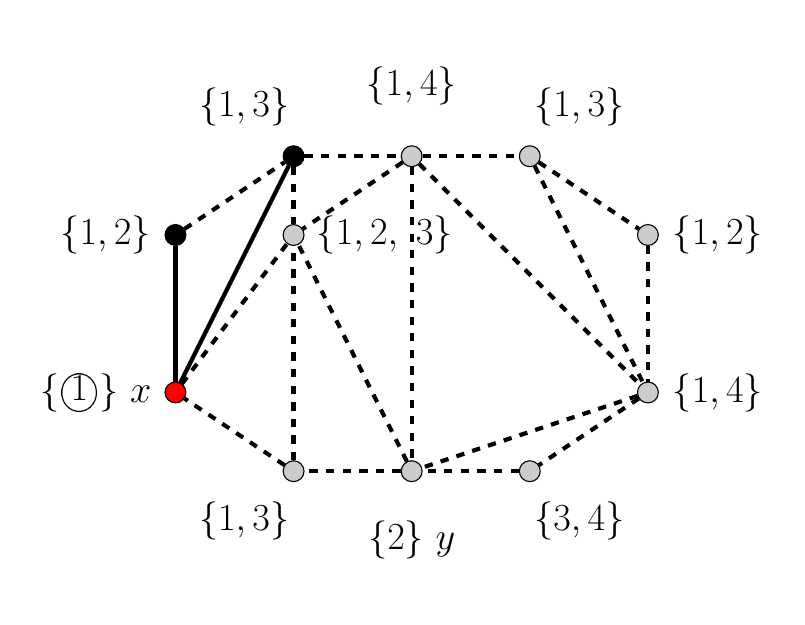
\begin{tikzpicture}[every edge/.append style={dashed}]
	\node (1) [label=left:{$\{1,2\}$}] at (-3.0cm, 1.0cm) {};
	\node (2) [label=above left:{$\{1,3\}$}] at (-1.5cm, 2.0cm) {};
	\node (3) [label=above:{$\{1,4\}$}, fill opacity=0.2] at (0.0cm, 2.0cm) {};
	\node (4) [label=above right:{$\{1,3\}$}, fill opacity=0.2] at (1.5cm, 2.0cm) {};
	\node (5) [label=right:{$\{1,2\}$}, fill opacity=0.2] at (3.0cm, 1.0cm) {};
	\node (6) [label=right:{$\{1,4\}$}, fill opacity=0.2] at (3.0cm, -1.0cm) {};
	\node (7) [label=below right:{$\{3,4\}$}, fill opacity=0.2] at (1.5cm, -2.0cm) {};
	\node (8) [label=below:{$\{2\} \ y$}, fill opacity=0.2] at (0.0cm, -2.0cm) {};
	\node (9) [label=below left:{$\{1,3\}$}, fill opacity=0.2] at (-1.5cm, -2.0cm) {};
	\node (10) [label=left:{$\{\textcircled{1}\} \ x$}, fill=red] at (-3.0cm, -1.0cm) {};
	\node (11) [label=right:{$\{1,2, \ 3\}$}, fill opacity=0.2] at (-1.5cm, 1.0cm) {};
	
	\draw (1) edge (2); \draw (2) edge (3); \draw (3) edge (4);
	\draw (4) edge (5); \draw (5) edge (6); \draw (6) edge (7);
	\draw (7) edge (8); \draw (8) edge (9); \draw (9) edge (10);
	\draw (10) edge [solid] (1);
	
	\draw (2) edge (11); \draw (3) edge (11); \draw (3) edge (6);
	\draw (4) edge (6); \draw (3) edge (8); \draw (6) edge (8);
	\draw (8) edge (11); \draw (9) edge (11); \draw (10) edge (11);
	\draw (10) edge [solid] (2);
\end{tikzpicture}
\end{center}
\end{frame}

\begin{frame}{Hartman-Skrekovski list-coloring}
\begin{center}
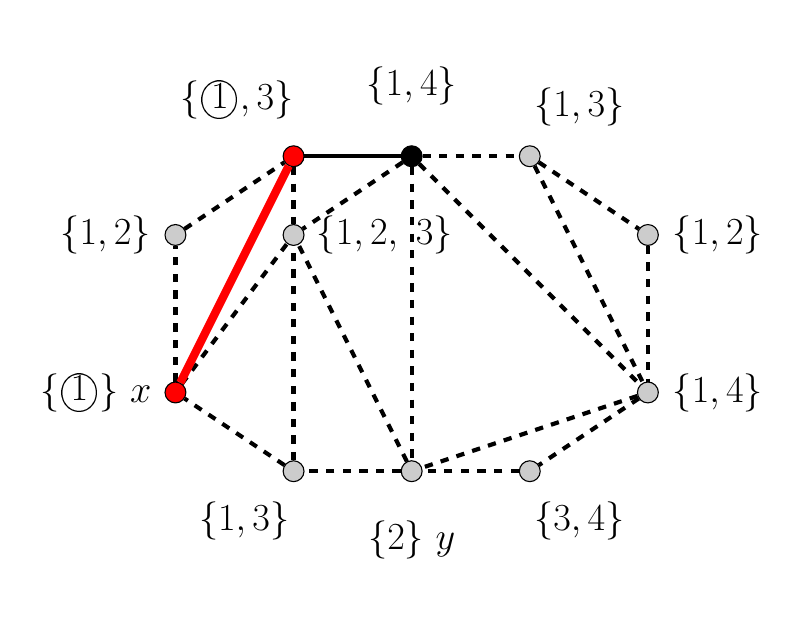
\begin{tikzpicture}[every edge/.append style={dashed}]
	\node (1) [label=left:{$\{1,2\}$}, fill opacity=0.2] at (-3.0cm, 1.0cm) {};
	\node (2) [label=above left:{$\{\textcircled{1},3\}$}, fill=red] at (-1.5cm, 2.0cm) {};
	\node (3) [label=above:{$\{1,4\}$}] at (0.0cm, 2.0cm) {};
	\node (4) [label=above right:{$\{1,3\}$}, fill opacity=0.2] at (1.5cm, 2.0cm) {};
	\node (5) [label=right:{$\{1,2\}$}, fill opacity=0.2] at (3.0cm, 1.0cm) {};
	\node (6) [label=right:{$\{1,4\}$}, fill opacity=0.2] at (3.0cm, -1.0cm) {};
	\node (7) [label=below right:{$\{3,4\}$}, fill opacity=0.2] at (1.5cm, -2.0cm) {};
	\node (8) [label=below:{$\{2\} \ y$}, fill opacity=0.2] at (0.0cm, -2.0cm) {};
	\node (9) [label=below left:{$\{1,3\}$}, fill opacity=0.2] at (-1.5cm, -2.0cm) {};
	\node (10) [label=left:{$\{\textcircled{1}\} \ x$}, fill=red] at (-3.0cm, -1.0cm) {};
	\node (11) [label=right:{$\{1,2, \ 3\}$}, fill opacity=0.2] at (-1.5cm, 1.0cm) {};
	
	\draw (1) edge (2); \draw (2) edge [solid] (3); \draw (3) edge (4);
	\draw (4) edge (5); \draw (5) edge (6); \draw (6) edge (7);
	\draw (7) edge (8); \draw (8) edge (9); \draw (9) edge (10);
	\draw (10) edge (1);
	
	\draw (2) edge (11); \draw (3) edge (11); \draw (3) edge (6);
	\draw (4) edge (6); \draw (3) edge (8); \draw (6) edge (8);
	\draw (8) edge (11); \draw (9) edge (11); \draw (10) edge (11);
	\draw (10) edge [line width=3pt, color=red, solid] (2);
\end{tikzpicture}
\end{center}
\end{frame}

\begin{frame}{Hartman-Skrekovski list-coloring}
\begin{center}
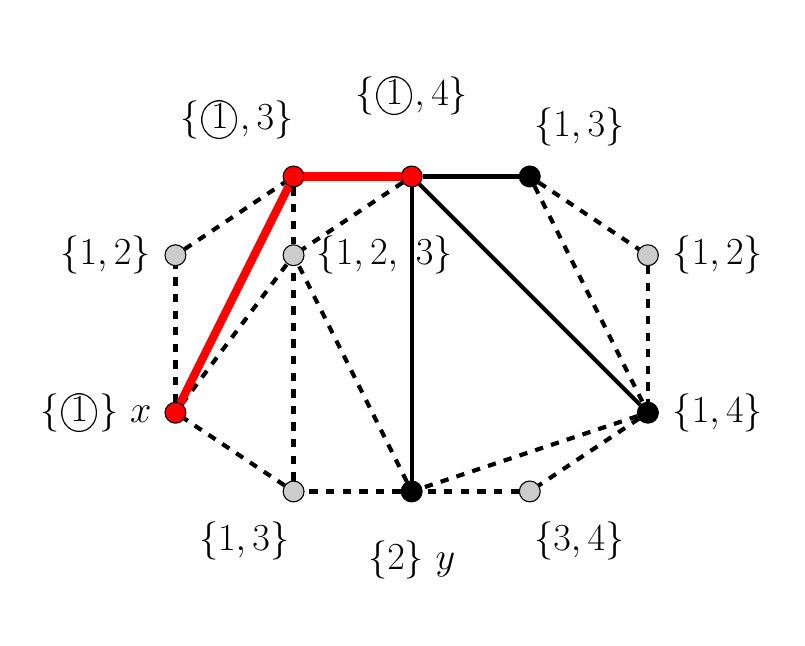
\begin{tikzpicture}[every edge/.append style={dashed}]
	\node (1) [label=left:{$\{1,2\}$}, fill opacity=0.2] at (-3.0cm, 1.0cm) {};
	\node (2) [label=above left:{$\{\textcircled{1},3\}$}, fill=red] at (-1.5cm, 2.0cm) {};
	\node (3) [label=above:{$\{\textcircled{1},4\}$}, fill=red] at (0.0cm, 2.0cm) {};
	\node (4) [label=above right:{$\{1,3\}$}] at (1.5cm, 2.0cm) {};
	\node (5) [label=right:{$\{1,2\}$}, fill opacity=0.2] at (3.0cm, 1.0cm) {};
	\node (6) [label=right:{$\{1,4\}$}] at (3.0cm, -1.0cm) {};
	\node (7) [label=below right:{$\{3,4\}$}, fill opacity=0.2] at (1.5cm, -2.0cm) {};
	\node (8) [label=below:{$\{2\} \ y$}] at (0.0cm, -2.0cm) {};
	\node (9) [label=below left:{$\{1,3\}$}, fill opacity=0.2] at (-1.5cm, -2.0cm) {};
	\node (10) [label=left:{$\{\textcircled{1}\} \ x$}, fill=red] at (-3.0cm, -1.0cm) {};
	\node (11) [label=right:{$\{1,2, \ 3\}$}, fill opacity=0.2] at (-1.5cm, 1.0cm) {};
	
	\draw (1) edge (2); \draw (2) edge [line width=3pt, color=red, solid] (3);
	\draw (3) edge [solid] (4);
	\draw (4) edge (5); \draw (5) edge (6); \draw (6) edge (7);
	\draw (7) edge (8); \draw (8) edge (9); \draw (9) edge (10);
	\draw (10) edge (1);
	
	\draw (2) edge (11); \draw (3) edge (11); \draw (3) edge [solid] (6);
	\draw (4) edge (6); \draw (3) edge [solid] (8); \draw (6) edge (8);
	\draw (8) edge (11); \draw (9) edge (11); \draw (10) edge (11);
	\draw (10) edge [line width=3pt, color=red, solid] (2);
\end{tikzpicture}
\end{center}
\end{frame}

\begin{frame}{Hartman-Skrekovski list-coloring}
\begin{center}
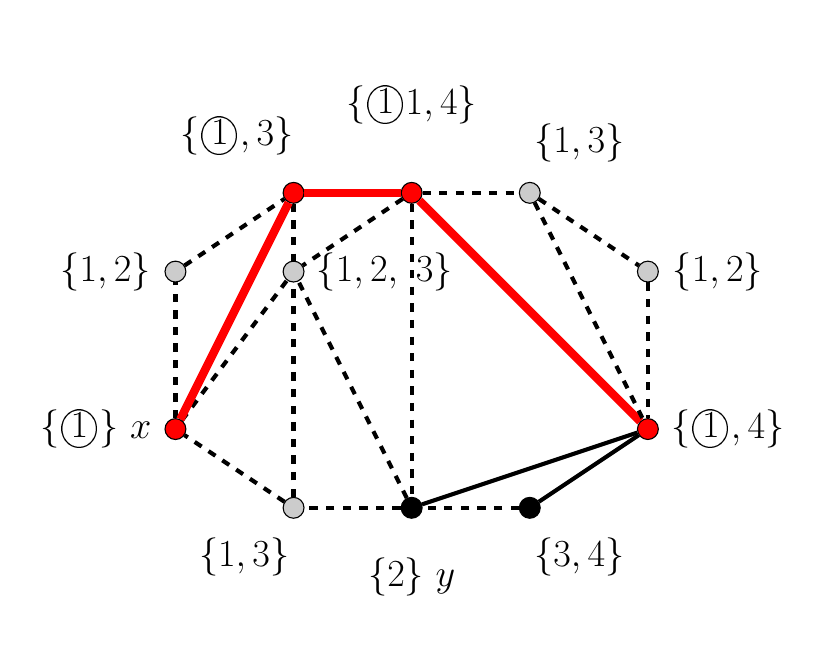
\begin{tikzpicture}[every edge/.append style={dashed}]
	\node (1) [label=left:{$\{1,2\}$}, fill opacity=0.2] at (-3.0cm, 1.0cm) {};
	\node (2) [label=above left:{$\{\textcircled{1},3\}$}, fill=red] at (-1.5cm, 2.0cm) {};
	\node (3) [label=above:{$\{\textcircled{1}1,4\}$}, fill=red] at (0.0cm, 2.0cm) {};
	\node (4) [label=above right:{$\{1,3\}$}, fill opacity=0.2] at (1.5cm, 2.0cm) {};
	\node (5) [label=right:{$\{1,2\}$}, fill opacity=0.2] at (3.0cm, 1.0cm) {};
	\node (6) [label=right:{$\{\textcircled{1},4\}$}, fill=red] at (3.0cm, -1.0cm) {};
	\node (7) [label=below right:{$\{3,4\}$}] at (1.5cm, -2.0cm) {};
	\node (8) [label=below:{$\{2\} \ y$}] at (0.0cm, -2.0cm) {};
	\node (9) [label=below left:{$\{1,3\}$}, fill opacity=0.2] at (-1.5cm, -2.0cm) {};
	\node (10) [label=left:{$\{\textcircled{1}\} \ x$}, fill=red] at (-3.0cm, -1.0cm) {};
	\node (11) [label=right:{$\{1,2, \ 3\}$}, fill opacity=0.2] at (-1.5cm, 1.0cm) {};
	
	\draw (1) edge (2); \draw (2) edge [line width=3pt, color=red, solid] (3);
	\draw (3) edge (4);
	\draw (4) edge (5); \draw (5) edge (6); \draw (6) edge [solid] (7);
	\draw (7) edge (8); \draw (8) edge (9); \draw (9) edge (10);
	\draw (10) edge (1);
	
	\draw (2) edge (11); \draw (3) edge (11);
	\draw (3) edge [line width=3pt, color=red, solid] (6);
	\draw (4) edge (6); \draw (3) edge (8); \draw (6) edge [solid] (8);
	\draw (8) edge (11); \draw (9) edge (11); \draw (10) edge (11);
	\draw (10) edge [line width=3pt, color=red, solid] (2);
\end{tikzpicture}
\end{center}
\end{frame}

\begin{frame}{Hartman-Skrekovski list-coloring}
\begin{center}
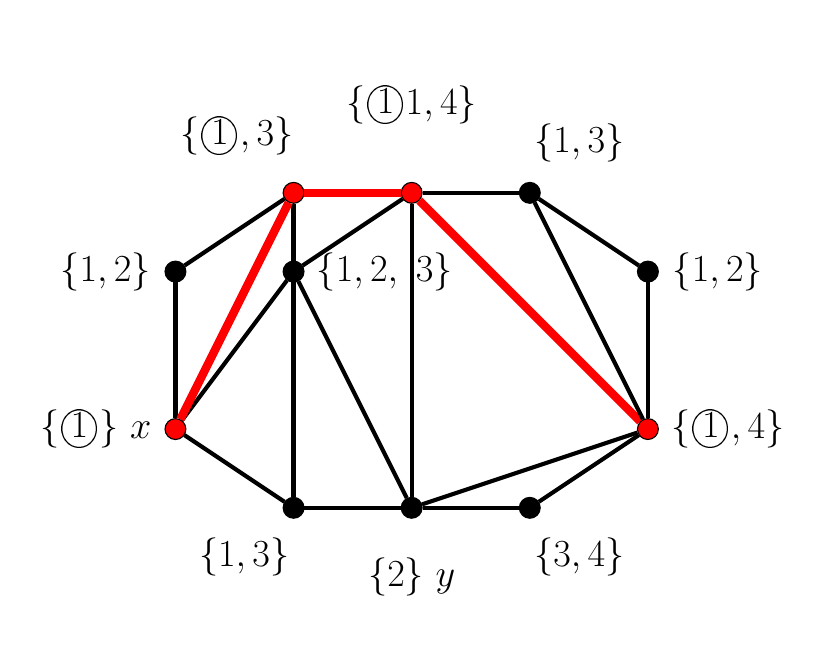
\begin{tikzpicture}
	\node (1) [label=left:{$\{1,2\}$}] at (-3.0cm, 1.0cm) {};
	\node (2) [label=above left:{$\{\textcircled{1},3\}$}, fill=red] at (-1.5cm, 2.0cm) {};
	\node (3) [label=above:{$\{\textcircled{1}1,4\}$}, fill=red] at (0.0cm, 2.0cm) {};
	\node (4) [label=above right:{$\{1,3\}$}] at (1.5cm, 2.0cm) {};
	\node (5) [label=right:{$\{1,2\}$}] at (3.0cm, 1.0cm) {};
	\node (6) [label=right:{$\{\textcircled{1},4\}$}, fill=red] at (3.0cm, -1.0cm) {};
	\node (7) [label=below right:{$\{3,4\}$}] at (1.5cm, -2.0cm) {};
	\node (8) [label=below:{$\{2\} \ y$}] at (0.0cm, -2.0cm) {};
	\node (9) [label=below left:{$\{1,3\}$}] at (-1.5cm, -2.0cm) {};
	\node (10) [label=left:{$\{\textcircled{1}\} \ x$}, fill=red] at (-3.0cm, -1.0cm) {};
	\node (11) [label=right:{$\{1,2, \ 3\}$}] at (-1.5cm, 1.0cm) {};
	
	\draw (1) edge (2); \draw (2) edge [line width=3pt, color=red] (3);
	\draw (3) edge (4);
	\draw (4) edge (5); \draw (5) edge (6); \draw (6) edge (7);
	\draw (7) edge (8); \draw (8) edge (9); \draw (9) edge (10);
	\draw (10) edge (1);
	
	\draw (2) edge (11); \draw (3) edge (11);
	\draw (3) edge [line width=3pt, color=red] (6);
	\draw (4) edge (6); \draw (3) edge (8); \draw (6) edge (8);
	\draw (8) edge (11); \draw (9) edge (11); \draw (10) edge (11);
	\draw (10) edge [line width=3pt, color=red] (2);
\end{tikzpicture}
\end{center}
\end{frame}


\begin{frame}{Hartman-Skrekovski list-coloring}
If an edge $uv$ of the path $P$ is not an edge of $C$ we will then separately
consider the two subgraphs formed by dividing along $uv$. The section not
containing $x$ and $y$ will be called a \textbf{lobe}.

We now have several weakly triangulated subgraphs, each with a path colored $c$
along their outer cycle.
\end{frame}

\begin{frame}{Hartman-Skrekovski list-coloring}
\begin{center}
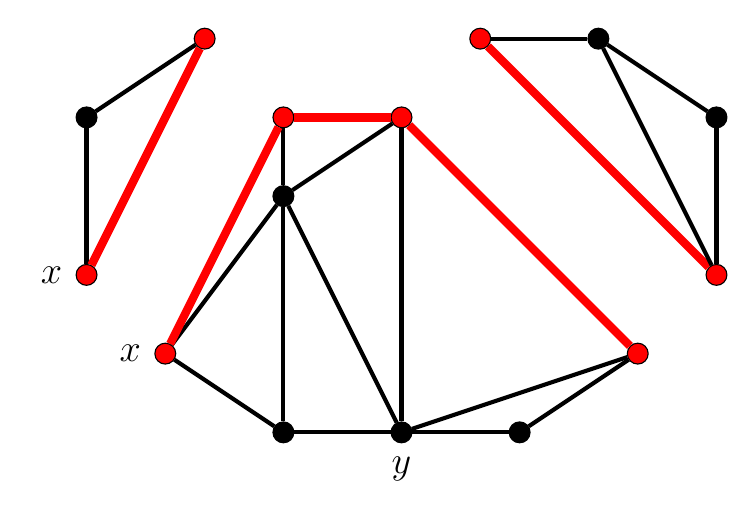
\begin{tikzpicture}
	\node (1) at (-4.0cm, 2.0cm) {};
	\node (10p) [label=left:$x$, fill=red] at (-4.0cm, 0.0cm) {};
	\node (2p) [fill=red] at (-2.5cm, 3.0cm) {};
	
	\node (4) at (2.5cm, 3.0cm) {};
	\node (5) at (4.0cm, 2.0cm) {};
	\node (3p) [fill=red] at (1.0cm, 3.0cm) {};
	\node (6p) [fill=red] at (4.0cm, 0.0cm) {};
	
	\node (2) [fill=red] at (-1.5cm, 2.0cm) {};
	\node (3) [fill=red] at (0.0cm, 2.0cm) {};
	\node (6) [fill=red] at (3.0cm, -1.0cm) {};
	\node (7) at (1.5cm, -2.0cm) {};
	\node (8) [label=below:$y$] at (0.0cm, -2.0cm) {};
	\node (9) at (-1.5cm, -2.0cm) {};
	\node (10) [label=left:$x$, fill=red] at (-3.0cm, -1.0cm) {};
	\node (11) at (-1.5cm, 1.0cm) {};
	
	\draw (1) edge (2p); \draw (2) edge [line width=3pt, color=red] (3);
	\draw (3p) edge (4);
	\draw (4) edge (5); \draw (5) edge (6p); \draw (6) edge (7);
	\draw (7) edge (8); \draw (8) edge (9); \draw (9) edge (10);
	\draw (10p) edge (1);
	\draw (10p) edge [line width=3pt, color=red] (2p);
	\draw (3p) edge [line width=3pt, color=red] (6p);
	
	\draw (2) edge (11); \draw (3) edge (11);
	\draw (3) edge [line width=3pt, color=red] (6);
	\draw (4) edge (6p); \draw (3) edge (8); \draw (6) edge (8);
	\draw (8) edge (11); \draw (9) edge (11); \draw (10) edge (11);
	\draw (10) edge [line width=3pt, color=red] (2);
\end{tikzpicture}
\end{center}
\end{frame}

\begin{frame}{Hartman-Skrekovski list-coloring}
We will now proceed to remove the colored path $P$ and update the color lists
of the remaining vertices so vertices with neighbors in $P$ will be colored $c$.

What remains will be several subgraphs with list assignments
such that we may separately apply the algorithm to color each.

We will now remove the colored path $P$. Also, for all vertices
$v$ adjacent to a vertex in $P$ we will remove $c$ from $L(v)$.
\end{frame}

\begin{frame}{Hartman-Skrekovski list-coloring}
\begin{center}
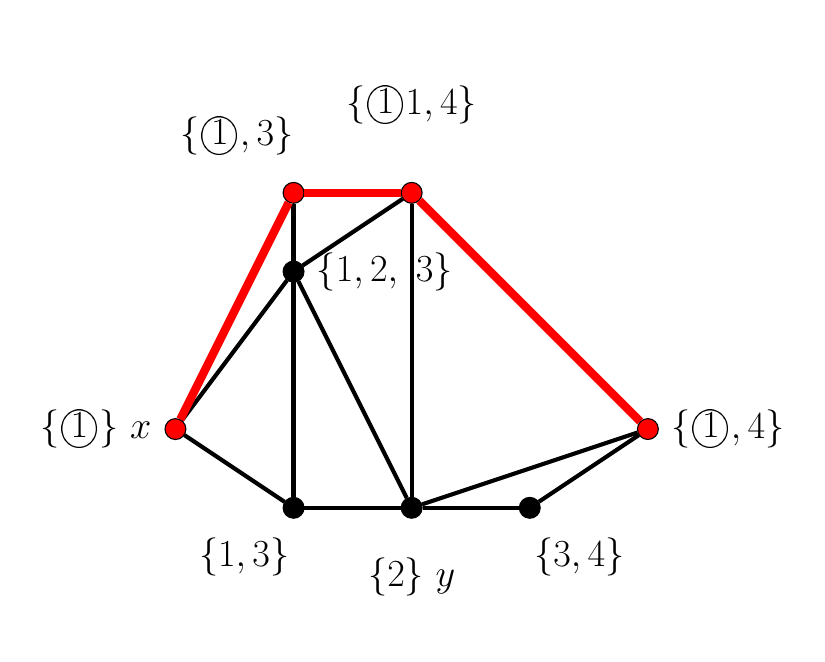
\begin{tikzpicture}
	\node (2) [label=above left:{$\{\textcircled{1},3\}$}, fill=red] at (-1.5cm, 2.0cm) {};
	\node (3) [label=above:{$\{\textcircled{1}1,4\}$}, fill=red] at (0.0cm, 2.0cm) {};
	\node (6) [label=right:{$\{\textcircled{1},4\}$}, fill=red] at (3.0cm, -1.0cm) {};
	\node (7) [label=below right:{$\{3,4\}$}] at (1.5cm, -2.0cm) {};
	\node (8) [label=below:{$\{2\} \ y$}] at (0.0cm, -2.0cm) {};
	\node (9) [label=below left:{$\{1,3\}$}] at (-1.5cm, -2.0cm) {};
	\node (10) [label=left:{$\{\textcircled{1}\} \ x$}, fill=red] at (-3.0cm, -1.0cm) {};
	\node (11) [label=right:{$\{1,2, \ 3\}$}] at (-1.5cm, 1.0cm) {};
	
	\draw (2) edge [line width=3pt, color=red] (3);
	\draw (6) edge (7);
	\draw (7) edge (8); \draw (8) edge (9); \draw (9) edge (10);
	
	\draw (2) edge (11); \draw (3) edge (11);
	\draw (3) edge [line width=3pt, color=red] (6);
	\draw (3) edge (8); \draw (6) edge (8);
	\draw (8) edge (11); \draw (9) edge (11); \draw (10) edge (11);
	\draw (10) edge [line width=3pt, color=red] (2);
\end{tikzpicture}
\end{center}
\end{frame}

\begin{frame}{Hartman-Skrekovski list-coloring}
\begin{center}
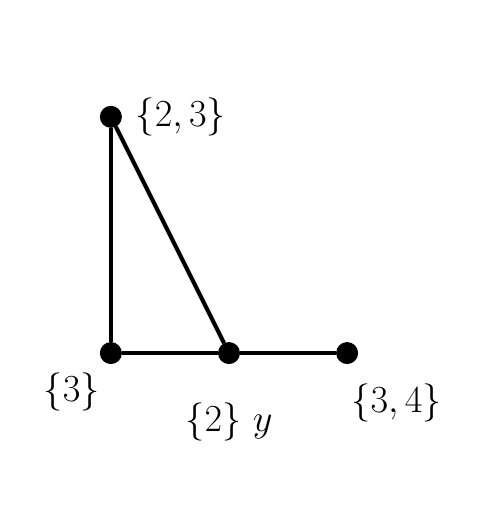
\begin{tikzpicture}
	\node (2) [draw=none,fill=none] at (-1.5cm, 2.0cm) {};
	\node (3) [draw=none,fill=none] at (0.0cm, 2.0cm) {};
	\node (6) [draw=none,fill=none] at (3.0cm, -1.0cm) {};
	\node (7) [label=below right:{$\{3,4\}$}] at (1.5cm, -2.0cm) {};
	\node (8) [label=below:{$\{2\} \ y$}] at (0.0cm, -2.0cm) {};
	\node (9) [label=below left:{$\{3\}$}] at (-1.5cm, -2.0cm) {};
	\node (11) [label=right:{$\{2,3\}$}] at (-1.5cm, 1.0cm) {};
	
	\draw (7) edge (8); \draw (8) edge (9);
	
	\draw (8) edge (11); \draw (9) edge (11);
\end{tikzpicture}
\end{center}
\end{frame}

\begin{frame}{Hartman-Skrekovski list-coloring}
The key idea that makes this work is that a vertex only ends up with one
remaining color in its list when it is in a position to be made $x$ or $y$ in
the recursive call.\\
\hfill\\

\begin{center}
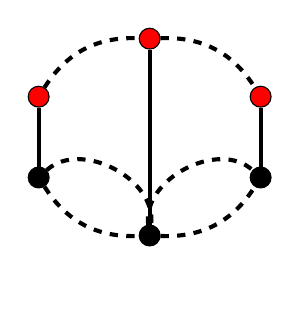
\begin{tikzpicture}
  \node (p0) [fill=red] at (160:1.5cm) {};
  \node (p1) [fill=red] at (90:1.25cm) {};
  \node (pn) [fill=red] at (20:1.5cm) {};
  \node (q0) at (200:1.5cm) {};
  \node (q1) at (270:1.25cm) {};
  \node (qn) at (340:1.5cm) {};
  \node (null) [fill=none,draw=none] at (270:1.75cm) {};
  
  \draw (p0) edge [bend left] (p1) [dashed];
  \draw (p1) edge [bend left] (pn) [dashed];
  \draw (q0) edge [bend right] (q1) [dashed];
  \draw (q1) edge [bend right] (qn) [dashed];
  \draw (q0) edge [bend left=70] (q1) [dashed];
  \draw (q1) edge [bend left=70] (qn) [dashed];
  \draw (p0) edge (q0);
  \draw (pn) edge (qn);
  \draw (p1) edge (q1);
\end{tikzpicture}
\end{center}
\end{frame}

\begin{frame}{Implementing Hartman-Skrekovski}
There are two main challenges faced in implementing Hartman and Skrekovski's
algorithm:
\begin{enumerate}
\item removing paths and locating remaining components;
\item tracking where vertices are on the outer face.
\end{enumerate}
\end{frame}

\begin{frame}{Implementing Hartman-Skrekovski}
\begin{prb}
We must remove a path and locate all the remaining subgraphs in order to make
recursive calls.
\end{prb}

\begin{ida}
We remove the path one vertex at a time and immediately make any recursive calls
as they become available.
\end{ida}
\end{frame}

\begin{frame}{Implementing Hartman-Skrekovski}
Suppose we are at the point in the algorithm where we have a cycle
$C=v_1v_2\ldots v_k$, and a colored path along the cycle.

Suppose $v_1$ is a path vertex we wish to remove. We will iterate through its neighbors
counterclockwise, starting with the neighbor $v_k$ and ending with the neighbor
$v_2$.

\begin{center}
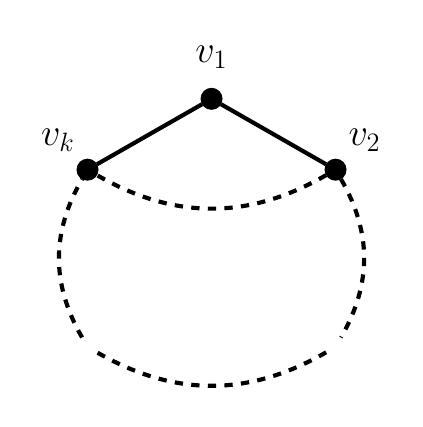
\begin{tikzpicture}[scale=0.9]
  \node (y) [draw=none,fill=none,minimum size=0mm] at (1.75cm,-1.25cm) {};
  
  \node (cn) [label=above left:$v_k$] at (-1.75cm,1.25cm) {};
  
  \node (p) [label=above:$v_1$] at (0cm,2.25cm) {};
  
  \node (c1) [label=above right:$v_2$] at (1.75cm,1.25cm) {};
  
  \node (x) [draw=none,fill=none,minimum size=0mm] at (-1.75cm,-1.25cm) {};
  
  \draw (y) edge [bend left] (x) [dashed];
  \draw (x) edge [bend left] (cn) [dashed];
  \draw (c1) edge [bend left] (y) [dashed];
  \draw (c1) edge [bend left] (cn) [dashed];
  \draw (cn) edge (p); \draw (p) edge (c1);
\end{tikzpicture}
\end{center}
\end{frame}

\begin{frame}{Implementing Hartman-Skrekovski}
At each neighbor we will remove the given color from their list if necessary.

If a neighbor is an interior vertex we will update vertex properties to note
that it is now on the outer face.

\begin{center}
\begin{tikzpicture}[scale=0.9]
  \node (y) [draw=none,fill=none,minimum size=0mm] at (1.75cm,-1.25cm) {};
  
  \node (cn) [label=above left:$v_k$] at (-1.75cm,1.25cm) {};
  
  \node (p) [label=above:$v_1$] at (0cm,2.25cm) {};
  
  \node (x) [draw=none,fill=none,minimum size=0mm] at (-1.75cm,-1.25cm) {};
  
  \node (c1) [label=above right:$v_2$] at (1.75cm,1.25cm) {};
  
  \draw (y) edge [bend left] (x) [dashed];
  \draw (x) edge [bend left] (cn) [dashed];
  \draw (c1) edge [bend left] (y) [dashed];
  \draw (c1) edge [bend left] (cn) [dashed];
  \draw (cn) edge (p); \draw (p) edge (c1);
\end{tikzpicture}
\end{center}
\end{frame}

\begin{frame}{Implementing Hartman-Skrekovski}
If we hit a neighbor $v_i$ on the outer face, observe $v_1$ has been completely
removed from $C_1$ then we make the recursive call on the cycle $C_1$. Since
$v_1$ has been completely removed from $C_1$ we will continue the process of
removing $v_1$ from the cycle $C_2$.

\begin{center}
\begin{tikzpicture}
  \node (c_n) [label=above left:$v_k$, fill] at (-1.5cm, 1.25cm) {};
  \node (p) [label=above:{$v_1$}] at (0cm, 2cm) {};
  \node (p_label) [draw=none, scale=0.8] at (0cm, 2cm) {};
  \node (c_1) [label=above:$v_2$, fill] at (1.5cm, 1.25cm) {};
  \node (c_i) [label=below:$v_i$, fill] at (0cm, -1cm) {};
  \node (G_0) [draw=none,fill=none] at (-0.75cm, 0.12cm) {$C_1$};
  \node (G_1) [draw=none,fill=none] at (0.7cm, 0.5cm) {$C_2$};
  \draw (c_i) edge [bend left] (c_n) [dashed];
  \draw (c_n) edge [bend left] (c_i) [dashed];
  \draw (c_n) edge (p);
  \draw (p) edge (c_1);
  \draw (p) edge (c_i);
  \draw (c_1) edge [bend left] (c_i) [dashed];
\end{tikzpicture}
\end{center}
\end{frame}

\begin{frame}{Implementing Hartman-Skrekovski}
\begin{prb}
We must track where all vertices on the outer face are in relation to $x$, $y$,
and the path $P$.
\end{prb}

\begin{ida}
We mark vertices along the outer cycle to denote which ``region" they are in.
\end{ida}

\begin{center}
\begin{tikzpicture}
  \node (p) [label=above:{$p$}, fill] at (90:1cm) {};
  \node (x) [label=below left:{$x$}, fill] at (210:1cm) {};
  \node (y) [label=below right:{$y$}, fill] at (330:1cm) {};
  \node (sp) [draw=none, fill=none] at (150:1.25cm) {$s_p$};
  \node (sy) [draw=none, fill=none] at (30:1.25cm) {$s_y$};
  \node (sy) [draw=none, fill=none] at (270:1.25cm) {$s_x$};
  \node (null) [draw=none,fill=none] at (270:1.5cm) {};
  \draw (p) edge [bend left] (y) [dashed];
  \draw (y) edge [bend left] (x) [dashed];
  \draw (x) edge [bend left] (p) [dashed];
\end{tikzpicture}
\end{center}
\end{frame}

\begin{frame}{Implementing Hartman-Skrekovski}
When the path has been entirely removed the segments
$s_p$ and $s_y$ are no longer separated by the colored path $P$.

Moreover, we are about to start coloring a new path along the outer face and
must treat $s_p$ as a part of $s_y$, that is, the segment between $x$ and $y$
clockwise along the outer face.

Walking along and remarking vertices is slow. Instead, we use a disjoint set
(or union find) structure to store the segment marks. Then, as two segments
are merged we may simply perform a union so both marks are treated the same.
\end{frame}

\begin{frame}{Hartman-Skrekovski time complexity}
These techniques combine into an algorithm where we walk through the adjacency list of
each vertex a fixed number of times, and perform a fixed number of
operations per neighbor.

Therefore the resulting implementation is $\mathcal{O}(n)$.
\end{frame}

\begin{frame}{Boost}
For the deliverable implementation I chose to use the C++ Boost Graph Library:

\begin{enumerate}
\item Boost is well maintained and kept up to date with the C++ standard;
\item the Boost Graph Library is designed for the implementation of graph algorithms;
\item Boost implements all the standard algorithms for embedding,
	drawing, and triangulating planar graphs.
\end{enumerate}
\end{frame}

\begin{frame}{Deliverables}
Documented implementations of the following algorithms in the Boost Graph Library
\begin{enumerate}
\item Poh path $3$-coloring with breadth first search;
\item Poh path $3$-coloring with faster path finding;
\item Hartman-Skrekovski path $3$-list-coloring.
\end{enumerate}

In addition, a writeup describing the correctness and complexity of the
implementation details for each algorithm.
\end{frame}

\begin{frame}{Timeline}
\textbf{December 2015:} Began reading papers and thinking about planar graphs

\textbf{January 2016:} Talk 1

\textbf{February 2016:} Completed a ``first draft" implementation of Poh's
algorithm in Boost

\textbf{March 2016:} Talk 2

\textbf{April - August 2016:} Completed Boost implementations of the Poh
and Hartman-Skrekovski algorithms

\textbf{February 2017 (today!):} Talk 3 

\textbf{March 2017:} Finalize writeup

\textbf{April - May 2017:} Turn in paperwork and graduate
\end{frame}

\end{document}
